\documentclass[twoside]{book}

% Packages required by doxygen
\usepackage{calc}
\usepackage{doxygen}
\usepackage{graphicx}
\usepackage[utf8]{inputenc}
\usepackage{makeidx}
\usepackage{multicol}
\usepackage{multirow}
\usepackage{textcomp}
\usepackage[table]{xcolor}

% Font selection
\usepackage[T1]{fontenc}
\usepackage{mathptmx}
\usepackage[scaled=.90]{helvet}
\usepackage{courier}
\usepackage{amssymb}
\usepackage{sectsty}
\renewcommand{\familydefault}{\sfdefault}
\allsectionsfont{%
  \fontseries{bc}\selectfont%
  \color{darkgray}%
}
\renewcommand{\DoxyLabelFont}{%
  \fontseries{bc}\selectfont%
  \color{darkgray}%
}

% Page & text layout
\usepackage{geometry}
\geometry{%
  a4paper,%
  top=2.5cm,%
  bottom=2.5cm,%
  left=2.5cm,%
  right=2.5cm%
}
\tolerance=750
\hfuzz=15pt
\hbadness=750
\setlength{\emergencystretch}{15pt}
\setlength{\parindent}{0cm}
\setlength{\parskip}{0.2cm}
\makeatletter
\renewcommand{\paragraph}{%
  \@startsection{paragraph}{4}{0ex}{-1.0ex}{1.0ex}{%
    \normalfont\normalsize\bfseries\SS@parafont%
  }%
}
\renewcommand{\subparagraph}{%
  \@startsection{subparagraph}{5}{0ex}{-1.0ex}{1.0ex}{%
    \normalfont\normalsize\bfseries\SS@subparafont%
  }%
}
\makeatother

% Headers & footers
\usepackage{fancyhdr}
\pagestyle{fancyplain}
\fancyhead[LE]{\fancyplain{}{\bfseries\thepage}}
\fancyhead[CE]{\fancyplain{}{}}
\fancyhead[RE]{\fancyplain{}{\bfseries\leftmark}}
\fancyhead[LO]{\fancyplain{}{\bfseries\rightmark}}
\fancyhead[CO]{\fancyplain{}{}}
\fancyhead[RO]{\fancyplain{}{\bfseries\thepage}}
\fancyfoot[LE]{\fancyplain{}{}}
\fancyfoot[CE]{\fancyplain{}{}}
\fancyfoot[RE]{\fancyplain{}{\bfseries\scriptsize Generated on Fri Feb 21 2014 06\-:59\-:37 for Chess by Doxygen }}
\fancyfoot[LO]{\fancyplain{}{\bfseries\scriptsize Generated on Fri Feb 21 2014 06\-:59\-:37 for Chess by Doxygen }}
\fancyfoot[CO]{\fancyplain{}{}}
\fancyfoot[RO]{\fancyplain{}{}}
\renewcommand{\footrulewidth}{0.4pt}
\renewcommand{\chaptermark}[1]{%
  \markboth{#1}{}%
}
\renewcommand{\sectionmark}[1]{%
  \markright{\thesection\ #1}%
}

% Indices & bibliography
\usepackage{natbib}
\usepackage[titles]{tocloft}
\setcounter{tocdepth}{3}
\setcounter{secnumdepth}{5}
\makeindex

% Hyperlinks (required, but should be loaded last)
\usepackage{ifpdf}
\ifpdf
  \usepackage[pdftex,pagebackref=true]{hyperref}
\else
  \usepackage[ps2pdf,pagebackref=true]{hyperref}
\fi
\hypersetup{%
  colorlinks=true,%
  linkcolor=blue,%
  citecolor=blue,%
  unicode%
}

% Custom commands
\newcommand{\clearemptydoublepage}{%
  \newpage{\pagestyle{empty}\cleardoublepage}%
}


%===== C O N T E N T S =====

\begin{document}

% Titlepage & ToC
\hypersetup{pageanchor=false}
\pagenumbering{roman}
\begin{titlepage}
\vspace*{7cm}
\begin{center}%
{\Large Chess \\[1ex]\large 1.\-2 }\\
\vspace*{1cm}
{\large Generated by Doxygen 1.8.6}\\
\vspace*{0.5cm}
{\small Fri Feb 21 2014 06:59:37}\\
\end{center}
\end{titlepage}
\clearemptydoublepage
\tableofcontents
\clearemptydoublepage
\pagenumbering{arabic}
\hypersetup{pageanchor=true}

%--- Begin generated contents ---
\chapter{Hierarchical Index}
\section{Class Hierarchy}
This inheritance list is sorted roughly, but not completely, alphabetically\-:\begin{DoxyCompactList}
\item \contentsline{section}{tests.\-All\-Tests}{\pageref{classtests_1_1_all_tests}}{}
\item \contentsline{section}{tests.\-Bishop\-Test}{\pageref{classtests_1_1_bishop_test}}{}
\item \contentsline{section}{tests.\-Board\-Test}{\pageref{classtests_1_1_board_test}}{}
\item \contentsline{section}{model.\-Chess}{\pageref{classmodel_1_1_chess}}{}
\item \contentsline{section}{view.\-Chess\-G\-U\-I}{\pageref{classview_1_1_chess_g_u_i}}{}
\item \contentsline{section}{tests.\-Chess\-Test}{\pageref{classtests_1_1_chess_test}}{}
\item Focus\-Listener\begin{DoxyCompactList}
\item \contentsline{section}{controller.\-Text\-Input}{\pageref{classcontroller_1_1_text_input}}{}
\end{DoxyCompactList}
\item \contentsline{section}{tests.\-King\-Test}{\pageref{classtests_1_1_king_test}}{}
\item \contentsline{section}{tests.\-Knight\-Test}{\pageref{classtests_1_1_knight_test}}{}
\item \contentsline{section}{tests.\-Pawn\-Test}{\pageref{classtests_1_1_pawn_test}}{}
\item \contentsline{section}{pieces.\-Piece}{\pageref{classpieces_1_1_piece}}{}
\begin{DoxyCompactList}
\item \contentsline{section}{pieces.\-Bishop}{\pageref{classpieces_1_1_bishop}}{}
\item \contentsline{section}{pieces.\-King}{\pageref{classpieces_1_1_king}}{}
\item \contentsline{section}{pieces.\-Knight}{\pageref{classpieces_1_1_knight}}{}
\item \contentsline{section}{pieces.\-Pawn}{\pageref{classpieces_1_1_pawn}}{}
\item \contentsline{section}{pieces.\-Queen}{\pageref{classpieces_1_1_queen}}{}
\item \contentsline{section}{pieces.\-Rock}{\pageref{classpieces_1_1_rock}}{}
\item \contentsline{section}{pieces.\-Rook}{\pageref{classpieces_1_1_rook}}{}
\item \contentsline{section}{pieces.\-Sentry}{\pageref{classpieces_1_1_sentry}}{}
\end{DoxyCompactList}
\item \contentsline{section}{tests.\-Piece\-Test}{\pageref{classtests_1_1_piece_test}}{}
\item \contentsline{section}{tests.\-Queen\-Test}{\pageref{classtests_1_1_queen_test}}{}
\item \contentsline{section}{tests.\-Rock\-Test}{\pageref{classtests_1_1_rock_test}}{}
\item \contentsline{section}{tests.\-Rook\-Test}{\pageref{classtests_1_1_rook_test}}{}
\item \contentsline{section}{tests.\-Sentry\-Test}{\pageref{classtests_1_1_sentry_test}}{}
\item \contentsline{section}{model.\-Space}{\pageref{classmodel_1_1_space}}{}
\item \contentsline{section}{controller.\-Spring\-Utilities}{\pageref{classcontroller_1_1_spring_utilities}}{}
\item \contentsline{section}{controller.\-User\-Input}{\pageref{classcontroller_1_1_user_input}}{}
\item \contentsline{section}{tests.\-User\-Input\-Test}{\pageref{classtests_1_1_user_input_test}}{}
\item Action\-Listener\begin{DoxyCompactList}
\item \contentsline{section}{controller.\-Text\-Input}{\pageref{classcontroller_1_1_text_input}}{}
\end{DoxyCompactList}
\item J\-Panel\begin{DoxyCompactList}
\item \contentsline{section}{controller.\-Text\-Input}{\pageref{classcontroller_1_1_text_input}}{}
\item \contentsline{section}{model.\-Board}{\pageref{classmodel_1_1_board}}{}
\end{DoxyCompactList}
\end{DoxyCompactList}

\chapter{Class Index}
\section{Class List}
Here are the classes, structs, unions and interfaces with brief descriptions\-:\begin{DoxyCompactList}
\item\contentsline{section}{\hyperlink{classtests_1_1_all_tests}{tests.\-All\-Tests} }{\pageref{classtests_1_1_all_tests}}{}
\item\contentsline{section}{\hyperlink{classpieces_1_1_bishop}{pieces.\-Bishop} }{\pageref{classpieces_1_1_bishop}}{}
\item\contentsline{section}{\hyperlink{classtests_1_1_bishop_test}{tests.\-Bishop\-Test} }{\pageref{classtests_1_1_bishop_test}}{}
\item\contentsline{section}{\hyperlink{classmodel_1_1_board}{model.\-Board} }{\pageref{classmodel_1_1_board}}{}
\item\contentsline{section}{\hyperlink{classtests_1_1_board_test}{tests.\-Board\-Test} }{\pageref{classtests_1_1_board_test}}{}
\item\contentsline{section}{\hyperlink{classmodel_1_1_chess}{model.\-Chess} }{\pageref{classmodel_1_1_chess}}{}
\item\contentsline{section}{\hyperlink{classview_1_1_chess_g_u_i}{view.\-Chess\-G\-U\-I} }{\pageref{classview_1_1_chess_g_u_i}}{}
\item\contentsline{section}{\hyperlink{classtests_1_1_chess_test}{tests.\-Chess\-Test} }{\pageref{classtests_1_1_chess_test}}{}
\item\contentsline{section}{\hyperlink{classpieces_1_1_king}{pieces.\-King} }{\pageref{classpieces_1_1_king}}{}
\item\contentsline{section}{\hyperlink{classtests_1_1_king_test}{tests.\-King\-Test} }{\pageref{classtests_1_1_king_test}}{}
\item\contentsline{section}{\hyperlink{classpieces_1_1_knight}{pieces.\-Knight} }{\pageref{classpieces_1_1_knight}}{}
\item\contentsline{section}{\hyperlink{classtests_1_1_knight_test}{tests.\-Knight\-Test} }{\pageref{classtests_1_1_knight_test}}{}
\item\contentsline{section}{\hyperlink{classpieces_1_1_pawn}{pieces.\-Pawn} }{\pageref{classpieces_1_1_pawn}}{}
\item\contentsline{section}{\hyperlink{classtests_1_1_pawn_test}{tests.\-Pawn\-Test} }{\pageref{classtests_1_1_pawn_test}}{}
\item\contentsline{section}{\hyperlink{classpieces_1_1_piece}{pieces.\-Piece} }{\pageref{classpieces_1_1_piece}}{}
\item\contentsline{section}{\hyperlink{classtests_1_1_piece_test}{tests.\-Piece\-Test} }{\pageref{classtests_1_1_piece_test}}{}
\item\contentsline{section}{\hyperlink{classpieces_1_1_queen}{pieces.\-Queen} }{\pageref{classpieces_1_1_queen}}{}
\item\contentsline{section}{\hyperlink{classtests_1_1_queen_test}{tests.\-Queen\-Test} }{\pageref{classtests_1_1_queen_test}}{}
\item\contentsline{section}{\hyperlink{classpieces_1_1_rock}{pieces.\-Rock} }{\pageref{classpieces_1_1_rock}}{}
\item\contentsline{section}{\hyperlink{classtests_1_1_rock_test}{tests.\-Rock\-Test} }{\pageref{classtests_1_1_rock_test}}{}
\item\contentsline{section}{\hyperlink{classpieces_1_1_rook}{pieces.\-Rook} }{\pageref{classpieces_1_1_rook}}{}
\item\contentsline{section}{\hyperlink{classtests_1_1_rook_test}{tests.\-Rook\-Test} }{\pageref{classtests_1_1_rook_test}}{}
\item\contentsline{section}{\hyperlink{classpieces_1_1_sentry}{pieces.\-Sentry} }{\pageref{classpieces_1_1_sentry}}{}
\item\contentsline{section}{\hyperlink{classtests_1_1_sentry_test}{tests.\-Sentry\-Test} }{\pageref{classtests_1_1_sentry_test}}{}
\item\contentsline{section}{\hyperlink{classmodel_1_1_space}{model.\-Space} }{\pageref{classmodel_1_1_space}}{}
\item\contentsline{section}{\hyperlink{classcontroller_1_1_spring_utilities}{controller.\-Spring\-Utilities} }{\pageref{classcontroller_1_1_spring_utilities}}{}
\item\contentsline{section}{\hyperlink{classcontroller_1_1_text_input}{controller.\-Text\-Input} }{\pageref{classcontroller_1_1_text_input}}{}
\item\contentsline{section}{\hyperlink{classcontroller_1_1_user_input}{controller.\-User\-Input} }{\pageref{classcontroller_1_1_user_input}}{}
\item\contentsline{section}{\hyperlink{classtests_1_1_user_input_test}{tests.\-User\-Input\-Test} }{\pageref{classtests_1_1_user_input_test}}{}
\end{DoxyCompactList}

\chapter{Class Documentation}
\hypertarget{classtests_1_1_all_tests}{\section{tests.\-All\-Tests Class Reference}
\label{classtests_1_1_all_tests}\index{tests.\-All\-Tests@{tests.\-All\-Tests}}
}


The documentation for this class was generated from the following file\-:\begin{DoxyCompactItemize}
\item 
src/tests/All\-Tests.\-java\end{DoxyCompactItemize}

\hypertarget{classpieces_1_1_bishop}{\section{pieces.\-Bishop Class Reference}
\label{classpieces_1_1_bishop}\index{pieces.\-Bishop@{pieces.\-Bishop}}
}
Inheritance diagram for pieces.\-Bishop\-:\begin{figure}[H]
\begin{center}
\leavevmode
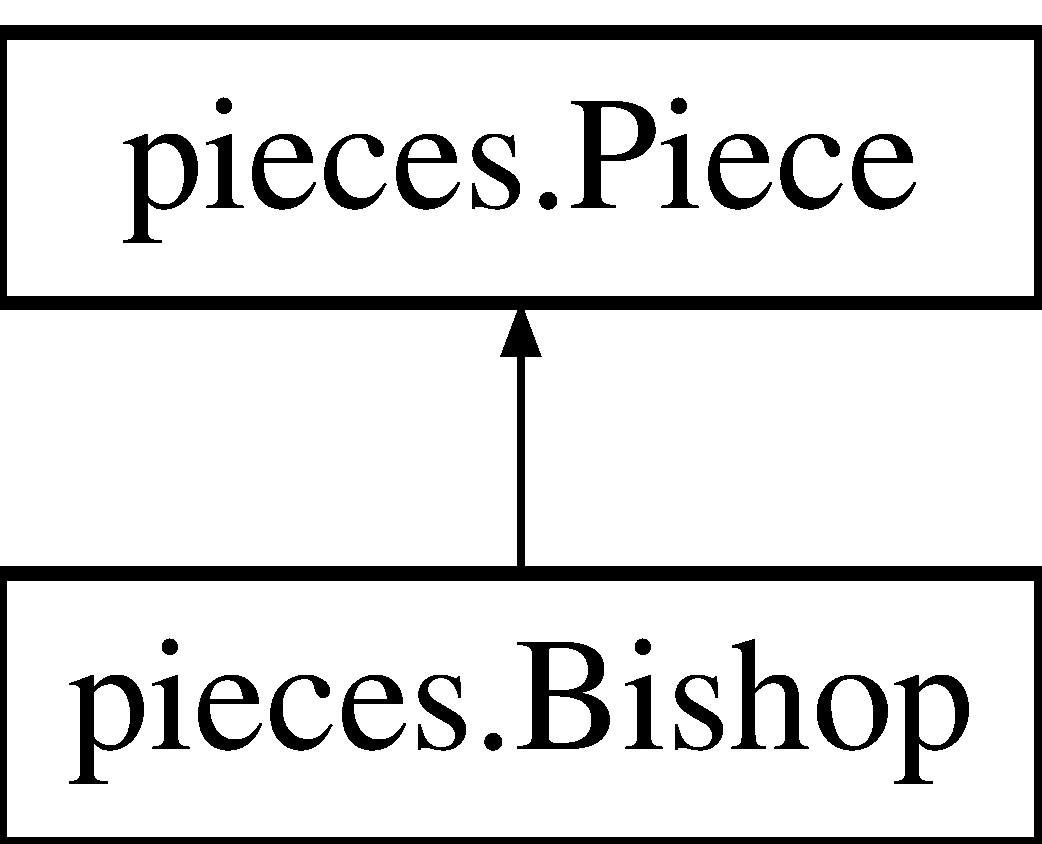
\includegraphics[height=2.000000cm]{classpieces_1_1_bishop}
\end{center}
\end{figure}
\subsection*{Public Member Functions}
\begin{DoxyCompactItemize}
\item 
void \hyperlink{classpieces_1_1_bishop_a81c18cc08e2ff3629418a961ae63fa72}{update\-Moves} (\hyperlink{classpieces_1_1_piece}{Piece}\mbox{[}$\,$\mbox{]}\mbox{[}$\,$\mbox{]} spaces, int rank, int file)
\end{DoxyCompactItemize}
\subsection*{Additional Inherited Members}


\subsection{Detailed Description}
\begin{DoxyAuthor}{Author}
Will 
\end{DoxyAuthor}


\subsection{Member Function Documentation}
\hypertarget{classpieces_1_1_bishop_a81c18cc08e2ff3629418a961ae63fa72}{\index{pieces\-::\-Bishop@{pieces\-::\-Bishop}!update\-Moves@{update\-Moves}}
\index{update\-Moves@{update\-Moves}!pieces::Bishop@{pieces\-::\-Bishop}}
\subsubsection[{update\-Moves}]{\setlength{\rightskip}{0pt plus 5cm}void pieces.\-Bishop.\-update\-Moves (
\begin{DoxyParamCaption}
\item[{{\bf Piece}}]{spaces\mbox{[}$\,$\mbox{]}\mbox{[}$\,$\mbox{]}, }
\item[{int}]{rank, }
\item[{int}]{file}
\end{DoxyParamCaption}
)}}\label{classpieces_1_1_bishop_a81c18cc08e2ff3629418a961ae63fa72}
Updates the possible moves for the piece. Bishops can only move diagonally. 
\begin{DoxyParams}{Parameters}
{\em spaces} & the current board state \\
\hline
{\em rank} & the x (rank) location of the piece \\
\hline
{\em file} & the y (file) location of the piece \\
\hline
\end{DoxyParams}


The documentation for this class was generated from the following file\-:\begin{DoxyCompactItemize}
\item 
src/pieces/Bishop.\-java\end{DoxyCompactItemize}

\hypertarget{classtests_1_1_bishop_test}{\section{tests.\-Bishop\-Test Class Reference}
\label{classtests_1_1_bishop_test}\index{tests.\-Bishop\-Test@{tests.\-Bishop\-Test}}
}
\subsection*{Public Member Functions}
\begin{DoxyCompactItemize}
\item 
\hypertarget{classtests_1_1_bishop_test_adeff634258715bf610ef1f657b0866f5}{void {\bfseries set\-Up} ()  throws Exception }\label{classtests_1_1_bishop_test_adeff634258715bf610ef1f657b0866f5}

\item 
\hypertarget{classtests_1_1_bishop_test_a628ea2649f6d7fdd7b6240a3a7de4597}{void {\bfseries bishop\-Move} ()}\label{classtests_1_1_bishop_test_a628ea2649f6d7fdd7b6240a3a7de4597}

\item 
\hypertarget{classtests_1_1_bishop_test_a4fe5bea5cde2887e3717600c654f2eab}{void {\bfseries horizontal\-Move} ()}\label{classtests_1_1_bishop_test_a4fe5bea5cde2887e3717600c654f2eab}

\item 
\hypertarget{classtests_1_1_bishop_test_a247b3d598a4d310bd23440ec1f63b1b0}{void {\bfseries vertical\-Move} ()}\label{classtests_1_1_bishop_test_a247b3d598a4d310bd23440ec1f63b1b0}

\item 
\hypertarget{classtests_1_1_bishop_test_aee47a6ff4e93a6454a431589b91a5e37}{void {\bfseries weird\-Move} ()}\label{classtests_1_1_bishop_test_aee47a6ff4e93a6454a431589b91a5e37}

\item 
\hypertarget{classtests_1_1_bishop_test_a8f7f82e6ee130181c90f57389c35a319}{void {\bfseries jump\-Friendly\-Pieces} ()}\label{classtests_1_1_bishop_test_a8f7f82e6ee130181c90f57389c35a319}

\item 
\hypertarget{classtests_1_1_bishop_test_ac98235f1eb576fdf224ed1b8469b088a}{void {\bfseries jump\-Enemy\-Pieces} ()}\label{classtests_1_1_bishop_test_ac98235f1eb576fdf224ed1b8469b088a}

\item 
\hypertarget{classtests_1_1_bishop_test_a6dbbfb5434f6826704e9e5b3cf443a6c}{void {\bfseries capture\-Friendly} ()}\label{classtests_1_1_bishop_test_a6dbbfb5434f6826704e9e5b3cf443a6c}

\item 
\hypertarget{classtests_1_1_bishop_test_a5378b093804f8755959dde2f98d82a64}{void {\bfseries capture\-Enemy} ()}\label{classtests_1_1_bishop_test_a5378b093804f8755959dde2f98d82a64}

\end{DoxyCompactItemize}


The documentation for this class was generated from the following file\-:\begin{DoxyCompactItemize}
\item 
src/tests/Bishop\-Test.\-java\end{DoxyCompactItemize}

\hypertarget{classmodel_1_1_board}{\section{model.\-Board Class Reference}
\label{classmodel_1_1_board}\index{model.\-Board@{model.\-Board}}
}
Inheritance diagram for model.\-Board\-:\begin{figure}[H]
\begin{center}
\leavevmode
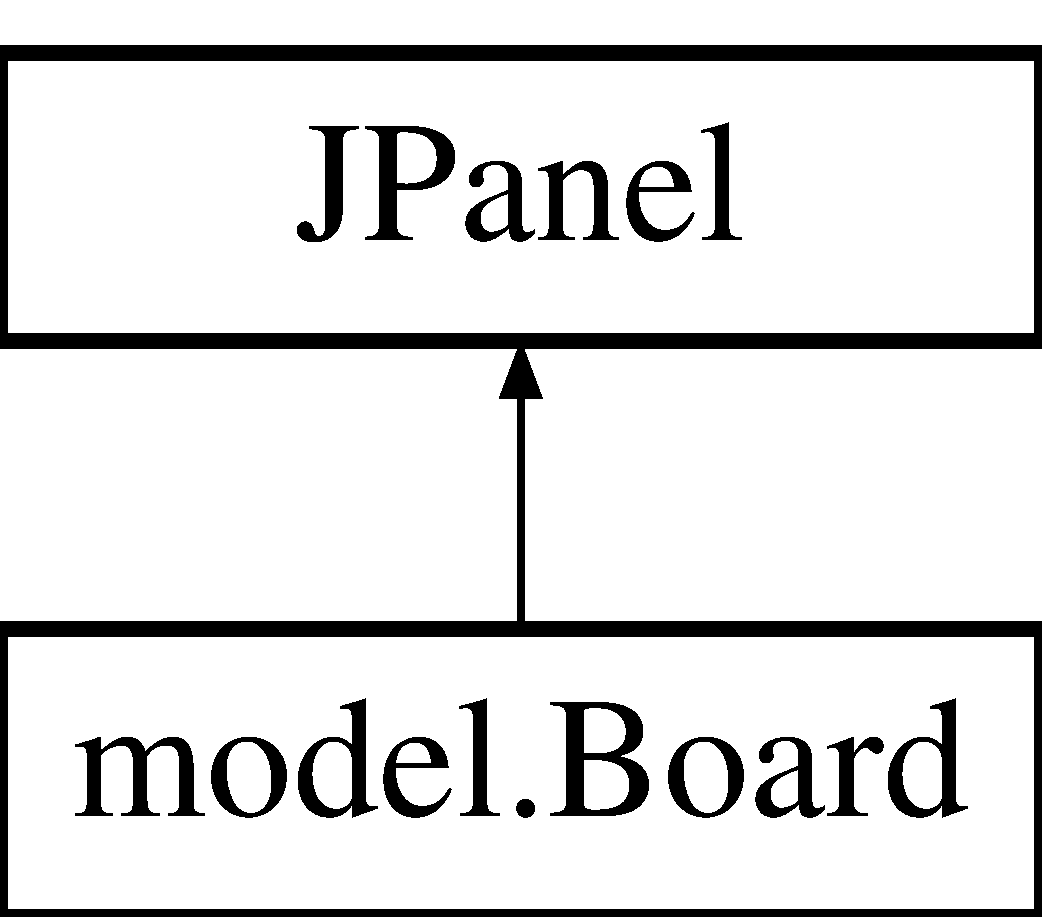
\includegraphics[height=2.000000cm]{classmodel_1_1_board}
\end{center}
\end{figure}
\subsection*{Public Member Functions}
\begin{DoxyCompactItemize}
\item 
\hyperlink{classmodel_1_1_board_aac7c0f18953f62b56fe1631dedc218ea}{Board} (\hyperlink{classmodel_1_1_board}{Board} other)
\item 
void \hyperlink{classmodel_1_1_board_ac230b4f661035db4d987134a91ab5cd4}{copy} (\hyperlink{classmodel_1_1_board}{Board} other)
\item 
void \hyperlink{classmodel_1_1_board_ab04268464780a556231843bfaca1f7bc}{reset} ()
\item 
void \hyperlink{classmodel_1_1_board_a00a494387b91835dbbc9c32ef253ca12}{paint\-Component} (Graphics g)
\item 
boolean \hyperlink{classmodel_1_1_board_a6578fe85a178404aa4da310dc28df012}{set\-Piece} (String piece, int rank, int file, Color player)
\item 
\hyperlink{classpieces_1_1_piece}{Piece} \hyperlink{classmodel_1_1_board_a516e546153648407b07174eeac9118d8}{get\-Piece} (int rank, int file)
\item 
boolean \hyperlink{classmodel_1_1_board_ad7df4bb61e00f8744f5593c2c8bd74a1}{move\-Piece} (int rstart, int fstart, int rtarget, int ftarget)
\item 
boolean \hyperlink{classmodel_1_1_board_aec15006cd7900c2b650b6f5dbeb35919}{out\-Of\-Bounds} (int rank, int file)
\item 
void \hyperlink{classmodel_1_1_board_ad96529c09bb3bef7dd29eae0a7d65cd8}{update\-Pieces} ()
\item 
boolean \hyperlink{classmodel_1_1_board_a55796d2d3a30e97826d734d79cde4d72}{in\-Check} (Color player)
\item 
boolean \hyperlink{classmodel_1_1_board_ae3d70f6d7bf853a60cbefb6872b73b3d}{in\-Checkmate} (Color player)
\item 
boolean \hyperlink{classmodel_1_1_board_a8758e5343f5a3dc5f965b622ebf012e3}{in\-Stalemate} (Color player)
\end{DoxyCompactItemize}


\subsection{Detailed Description}
\begin{DoxyAuthor}{Author}
Will 
\end{DoxyAuthor}


\subsection{Constructor \& Destructor Documentation}
\hypertarget{classmodel_1_1_board_aac7c0f18953f62b56fe1631dedc218ea}{\index{model\-::\-Board@{model\-::\-Board}!Board@{Board}}
\index{Board@{Board}!model::Board@{model\-::\-Board}}
\subsubsection[{Board}]{\setlength{\rightskip}{0pt plus 5cm}model.\-Board.\-Board (
\begin{DoxyParamCaption}
\item[{{\bf Board}}]{other}
\end{DoxyParamCaption}
)}}\label{classmodel_1_1_board_aac7c0f18953f62b56fe1631dedc218ea}
Copy constructor 
\begin{DoxyParams}{Parameters}
{\em other} & the board to copy \\
\hline
\end{DoxyParams}


\subsection{Member Function Documentation}
\hypertarget{classmodel_1_1_board_ac230b4f661035db4d987134a91ab5cd4}{\index{model\-::\-Board@{model\-::\-Board}!copy@{copy}}
\index{copy@{copy}!model::Board@{model\-::\-Board}}
\subsubsection[{copy}]{\setlength{\rightskip}{0pt plus 5cm}void model.\-Board.\-copy (
\begin{DoxyParamCaption}
\item[{{\bf Board}}]{other}
\end{DoxyParamCaption}
)}}\label{classmodel_1_1_board_ac230b4f661035db4d987134a91ab5cd4}
A copy helper function that performs a deep copy of every element in the other board. 
\begin{DoxyParams}{Parameters}
{\em other} & \\
\hline
\end{DoxyParams}
\hypertarget{classmodel_1_1_board_a516e546153648407b07174eeac9118d8}{\index{model\-::\-Board@{model\-::\-Board}!get\-Piece@{get\-Piece}}
\index{get\-Piece@{get\-Piece}!model::Board@{model\-::\-Board}}
\subsubsection[{get\-Piece}]{\setlength{\rightskip}{0pt plus 5cm}{\bf Piece} model.\-Board.\-get\-Piece (
\begin{DoxyParamCaption}
\item[{int}]{rank, }
\item[{int}]{file}
\end{DoxyParamCaption}
)}}\label{classmodel_1_1_board_a516e546153648407b07174eeac9118d8}

\begin{DoxyParams}{Parameters}
{\em rank} & the x (rank) location of the piece \\
\hline
{\em file} & the y (file) location of the piece \\
\hline
\end{DoxyParams}
\begin{DoxyReturn}{Returns}
the piece at a given space 
\end{DoxyReturn}
\hypertarget{classmodel_1_1_board_a55796d2d3a30e97826d734d79cde4d72}{\index{model\-::\-Board@{model\-::\-Board}!in\-Check@{in\-Check}}
\index{in\-Check@{in\-Check}!model::Board@{model\-::\-Board}}
\subsubsection[{in\-Check}]{\setlength{\rightskip}{0pt plus 5cm}boolean model.\-Board.\-in\-Check (
\begin{DoxyParamCaption}
\item[{Color}]{player}
\end{DoxyParamCaption}
)}}\label{classmodel_1_1_board_a55796d2d3a30e97826d734d79cde4d72}

\begin{DoxyParams}{Parameters}
{\em player} & the color of the player check for check \\
\hline
\end{DoxyParams}
\begin{DoxyReturn}{Returns}
true if the given player is in check 
\end{DoxyReturn}
\hypertarget{classmodel_1_1_board_ae3d70f6d7bf853a60cbefb6872b73b3d}{\index{model\-::\-Board@{model\-::\-Board}!in\-Checkmate@{in\-Checkmate}}
\index{in\-Checkmate@{in\-Checkmate}!model::Board@{model\-::\-Board}}
\subsubsection[{in\-Checkmate}]{\setlength{\rightskip}{0pt plus 5cm}boolean model.\-Board.\-in\-Checkmate (
\begin{DoxyParamCaption}
\item[{Color}]{player}
\end{DoxyParamCaption}
)}}\label{classmodel_1_1_board_ae3d70f6d7bf853a60cbefb6872b73b3d}

\begin{DoxyParams}{Parameters}
{\em player} & the color of the player to check for checkmate \\
\hline
\end{DoxyParams}
\begin{DoxyReturn}{Returns}
true if the given player is in checkmate 
\end{DoxyReturn}
\hypertarget{classmodel_1_1_board_a8758e5343f5a3dc5f965b622ebf012e3}{\index{model\-::\-Board@{model\-::\-Board}!in\-Stalemate@{in\-Stalemate}}
\index{in\-Stalemate@{in\-Stalemate}!model::Board@{model\-::\-Board}}
\subsubsection[{in\-Stalemate}]{\setlength{\rightskip}{0pt plus 5cm}boolean model.\-Board.\-in\-Stalemate (
\begin{DoxyParamCaption}
\item[{Color}]{player}
\end{DoxyParamCaption}
)}}\label{classmodel_1_1_board_a8758e5343f5a3dc5f965b622ebf012e3}

\begin{DoxyParams}{Parameters}
{\em player} & the color of player to check for stalemate \\
\hline
\end{DoxyParams}
\begin{DoxyReturn}{Returns}
true if in stalemate 
\end{DoxyReturn}
\hypertarget{classmodel_1_1_board_ad7df4bb61e00f8744f5593c2c8bd74a1}{\index{model\-::\-Board@{model\-::\-Board}!move\-Piece@{move\-Piece}}
\index{move\-Piece@{move\-Piece}!model::Board@{model\-::\-Board}}
\subsubsection[{move\-Piece}]{\setlength{\rightskip}{0pt plus 5cm}boolean model.\-Board.\-move\-Piece (
\begin{DoxyParamCaption}
\item[{int}]{rstart, }
\item[{int}]{fstart, }
\item[{int}]{rtarget, }
\item[{int}]{ftarget}
\end{DoxyParamCaption}
)}}\label{classmodel_1_1_board_ad7df4bb61e00f8744f5593c2c8bd74a1}
Moves a piece on the board from (rstart,fstart) to (rtarget,ftarget). 
\begin{DoxyParams}{Parameters}
{\em rstart} & the starting rank (x position) of the move \\
\hline
{\em fstart} & the starting file (y position) of the move \\
\hline
{\em rtarget} & the target rank (x position) of the move \\
\hline
{\em ftarget} & the target file (y position) of the move \\
\hline
\end{DoxyParams}
\begin{DoxyReturn}{Returns}
true if the move was successful false otherwise 
\end{DoxyReturn}
\hypertarget{classmodel_1_1_board_aec15006cd7900c2b650b6f5dbeb35919}{\index{model\-::\-Board@{model\-::\-Board}!out\-Of\-Bounds@{out\-Of\-Bounds}}
\index{out\-Of\-Bounds@{out\-Of\-Bounds}!model::Board@{model\-::\-Board}}
\subsubsection[{out\-Of\-Bounds}]{\setlength{\rightskip}{0pt plus 5cm}boolean model.\-Board.\-out\-Of\-Bounds (
\begin{DoxyParamCaption}
\item[{int}]{rank, }
\item[{int}]{file}
\end{DoxyParamCaption}
)}}\label{classmodel_1_1_board_aec15006cd7900c2b650b6f5dbeb35919}
Checks whether a given (rank,file) pair is within the board range. 
\begin{DoxyParams}{Parameters}
{\em rank} & the x (rank) location of the piece \\
\hline
{\em file} & the y (file) location of the piece \\
\hline
\end{DoxyParams}
\begin{DoxyReturn}{Returns}
true if the position given is not a valid board position. 
\end{DoxyReturn}
\hypertarget{classmodel_1_1_board_a00a494387b91835dbbc9c32ef253ca12}{\index{model\-::\-Board@{model\-::\-Board}!paint\-Component@{paint\-Component}}
\index{paint\-Component@{paint\-Component}!model::Board@{model\-::\-Board}}
\subsubsection[{paint\-Component}]{\setlength{\rightskip}{0pt plus 5cm}void model.\-Board.\-paint\-Component (
\begin{DoxyParamCaption}
\item[{Graphics}]{g}
\end{DoxyParamCaption}
)}}\label{classmodel_1_1_board_a00a494387b91835dbbc9c32ef253ca12}
\begin{DoxySeeAlso}{See Also}
javax.\-swing.\-J\-Component\-::paint\-Component(java.\-awt.\-Graphics) 
\end{DoxySeeAlso}

\begin{DoxyParams}{Parameters}
{\em g} & the graphics element to paint the board onto \\
\hline
\end{DoxyParams}
\hypertarget{classmodel_1_1_board_ab04268464780a556231843bfaca1f7bc}{\index{model\-::\-Board@{model\-::\-Board}!reset@{reset}}
\index{reset@{reset}!model::Board@{model\-::\-Board}}
\subsubsection[{reset}]{\setlength{\rightskip}{0pt plus 5cm}void model.\-Board.\-reset (
\begin{DoxyParamCaption}
{}
\end{DoxyParamCaption}
)}}\label{classmodel_1_1_board_ab04268464780a556231843bfaca1f7bc}
Restarts the current board to the unitialized state with no pieces. \hypertarget{classmodel_1_1_board_a6578fe85a178404aa4da310dc28df012}{\index{model\-::\-Board@{model\-::\-Board}!set\-Piece@{set\-Piece}}
\index{set\-Piece@{set\-Piece}!model::Board@{model\-::\-Board}}
\subsubsection[{set\-Piece}]{\setlength{\rightskip}{0pt plus 5cm}boolean model.\-Board.\-set\-Piece (
\begin{DoxyParamCaption}
\item[{String}]{piece, }
\item[{int}]{rank, }
\item[{int}]{file, }
\item[{Color}]{player}
\end{DoxyParamCaption}
)}}\label{classmodel_1_1_board_a6578fe85a178404aa4da310dc28df012}

\begin{DoxyParams}{Parameters}
{\em piece} & the piece to set \\
\hline
{\em rank} & the x (rank) location of the piece \\
\hline
{\em file} & the y (file) location of the piece \\
\hline
{\em player} & the owner of the piece (W\-H\-I\-T\-E,B\-L\-A\-C\-K) \\
\hline
\end{DoxyParams}
\begin{DoxyReturn}{Returns}
true if the piece was set successfully 
\end{DoxyReturn}
\hypertarget{classmodel_1_1_board_ad96529c09bb3bef7dd29eae0a7d65cd8}{\index{model\-::\-Board@{model\-::\-Board}!update\-Pieces@{update\-Pieces}}
\index{update\-Pieces@{update\-Pieces}!model::Board@{model\-::\-Board}}
\subsubsection[{update\-Pieces}]{\setlength{\rightskip}{0pt plus 5cm}void model.\-Board.\-update\-Pieces (
\begin{DoxyParamCaption}
{}
\end{DoxyParamCaption}
)}}\label{classmodel_1_1_board_ad96529c09bb3bef7dd29eae0a7d65cd8}
We need to maintain possible moves for each piece to detect game-\/ending conditions. 

The documentation for this class was generated from the following file\-:\begin{DoxyCompactItemize}
\item 
src/model/Board.\-java\end{DoxyCompactItemize}

\hypertarget{classtests_1_1_board_test}{\section{tests.\-Board\-Test Class Reference}
\label{classtests_1_1_board_test}\index{tests.\-Board\-Test@{tests.\-Board\-Test}}
}
\subsection*{Public Member Functions}
\begin{DoxyCompactItemize}
\item 
\hypertarget{classtests_1_1_board_test_aa4971a32f439d2f67389bece2188dbcb}{void {\bfseries set\-Up} ()}\label{classtests_1_1_board_test_aa4971a32f439d2f67389bece2188dbcb}

\item 
\hypertarget{classtests_1_1_board_test_a49f3b5804a7cfed3694c2f8271a05a00}{void {\bfseries empty\-Constructor} ()}\label{classtests_1_1_board_test_a49f3b5804a7cfed3694c2f8271a05a00}

\item 
\hypertarget{classtests_1_1_board_test_acc9d9fa00e3ba979f9f04c35dcd81804}{void {\bfseries not\-In\-Check} ()}\label{classtests_1_1_board_test_acc9d9fa00e3ba979f9f04c35dcd81804}

\item 
\hypertarget{classtests_1_1_board_test_a0bfa72527d05a54277a27a836852fa38}{void {\bfseries not\-In\-Friendly\-Check} ()}\label{classtests_1_1_board_test_a0bfa72527d05a54277a27a836852fa38}

\item 
\hypertarget{classtests_1_1_board_test_a49cb96d5a1c4226909eb206886f5efe2}{void {\bfseries opponent\-In\-Check} ()}\label{classtests_1_1_board_test_a49cb96d5a1c4226909eb206886f5efe2}

\item 
\hypertarget{classtests_1_1_board_test_a82597a3ce2954e6dc0455935a5afb6ae}{void {\bfseries move\-Into\-Check} ()}\label{classtests_1_1_board_test_a82597a3ce2954e6dc0455935a5afb6ae}

\item 
\hypertarget{classtests_1_1_board_test_a746ead936beecae91bff6cb7a7a559cb}{void {\bfseries other\-Piece\-In\-Check} ()}\label{classtests_1_1_board_test_a746ead936beecae91bff6cb7a7a559cb}

\item 
\hypertarget{classtests_1_1_board_test_a255c1c93dc99704f27cbc9b5f6204a7f}{void {\bfseries capture\-Outof\-Check} ()}\label{classtests_1_1_board_test_a255c1c93dc99704f27cbc9b5f6204a7f}

\item 
\hypertarget{classtests_1_1_board_test_a1590c4d651a53644965518c73a697fe3}{void {\bfseries capture\-Into\-Check} ()}\label{classtests_1_1_board_test_a1590c4d651a53644965518c73a697fe3}

\item 
\hypertarget{classtests_1_1_board_test_a243ee277c9b08eb5f4b43374b5515675}{void {\bfseries empty\-Board\-Check} ()}\label{classtests_1_1_board_test_a243ee277c9b08eb5f4b43374b5515675}

\item 
\hypertarget{classtests_1_1_board_test_a3faa0906be350af3f3c60539e3a8c128}{void {\bfseries not\-In\-Friendly\-Checkmate} ()}\label{classtests_1_1_board_test_a3faa0906be350af3f3c60539e3a8c128}

\item 
\hypertarget{classtests_1_1_board_test_ac27f1707350258b2f9d1592e207ac06e}{void {\bfseries opponent\-In\-Checkmate} ()}\label{classtests_1_1_board_test_ac27f1707350258b2f9d1592e207ac06e}

\item 
\hypertarget{classtests_1_1_board_test_a5332c3c5c70faefe1931381651585884}{void {\bfseries not\-In\-Check\-Or\-Check\-Mate} ()}\label{classtests_1_1_board_test_a5332c3c5c70faefe1931381651585884}

\item 
\hypertarget{classtests_1_1_board_test_aadd0559f3c497349fa2aeadb36e2d5ae}{void {\bfseries not\-In\-Check\-Mate} ()}\label{classtests_1_1_board_test_aadd0559f3c497349fa2aeadb36e2d5ae}

\item 
\hypertarget{classtests_1_1_board_test_a84fd04ef00dbad620eb25b021bf7644d}{void {\bfseries empyt\-Board\-Check\-Mate} ()}\label{classtests_1_1_board_test_a84fd04ef00dbad620eb25b021bf7644d}

\item 
\hypertarget{classtests_1_1_board_test_a344e6649751aa23e9348e01fa80cdcac}{void {\bfseries in\-Stalemate} ()}\label{classtests_1_1_board_test_a344e6649751aa23e9348e01fa80cdcac}

\item 
\hypertarget{classtests_1_1_board_test_a07d70bc7e1ecec12347be2944af5666d}{void {\bfseries empty\-Board\-Stalemate} ()}\label{classtests_1_1_board_test_a07d70bc7e1ecec12347be2944af5666d}

\item 
\hypertarget{classtests_1_1_board_test_abea75be6399be67b5a408ea67644156e}{void {\bfseries no\-Stalemate\-In\-Check} ()}\label{classtests_1_1_board_test_abea75be6399be67b5a408ea67644156e}

\item 
\hypertarget{classtests_1_1_board_test_acd515721e7858ceccc6a508db6d5667e}{void {\bfseries no\-Check\-No\-Stalemate} ()}\label{classtests_1_1_board_test_acd515721e7858ceccc6a508db6d5667e}

\end{DoxyCompactItemize}


The documentation for this class was generated from the following file\-:\begin{DoxyCompactItemize}
\item 
src/tests/Board\-Test.\-java\end{DoxyCompactItemize}

\hypertarget{classmodel_1_1_chess}{\section{model.\-Chess Class Reference}
\label{classmodel_1_1_chess}\index{model.\-Chess@{model.\-Chess}}
}
\subsection*{Static Public Member Functions}
\begin{DoxyCompactItemize}
\item 
static void \hyperlink{classmodel_1_1_chess_aee53a6846e5dbe60cfd0b62cbe373788}{restart} ()
\item 
\hypertarget{classmodel_1_1_chess_ab7d140bf0b52b8397858de46fdf2a0ce}{static void {\bfseries wins} ()}\label{classmodel_1_1_chess_ab7d140bf0b52b8397858de46fdf2a0ce}

\item 
static void \hyperlink{classmodel_1_1_chess_af399b48ddd8715c973c47e495d4b3c25}{forfeit} ()
\item 
static void \hyperlink{classmodel_1_1_chess_a07b47f12039f14faa2328596cd0f06f6}{draw} ()
\item 
static Color \hyperlink{classmodel_1_1_chess_a6cd0aad82f26cb7db49848d977cd4b56}{get\-Turn} ()
\item 
static String \hyperlink{classmodel_1_1_chess_abd2d0e384c5be0d5195c05cc691364e1}{current\-Player} ()
\item 
static void \hyperlink{classmodel_1_1_chess_ab0062f08be39cde173dde158d1faacbe}{next\-Turn} ()
\item 
static String \hyperlink{classmodel_1_1_chess_a88168b5d5a7fd11c21d1132110da6e70}{get\-Score\-List} ()
\item 
static void \hyperlink{classmodel_1_1_chess_a060f443a73a9090f8160ea803e56f786}{set\-Player\-Names} (String\mbox{[}$\,$\mbox{]} players)
\end{DoxyCompactItemize}


\subsection{Detailed Description}
\begin{DoxyAuthor}{Author}
Will 
\end{DoxyAuthor}


\subsection{Member Function Documentation}
\hypertarget{classmodel_1_1_chess_abd2d0e384c5be0d5195c05cc691364e1}{\index{model\-::\-Chess@{model\-::\-Chess}!current\-Player@{current\-Player}}
\index{current\-Player@{current\-Player}!model::Chess@{model\-::\-Chess}}
\subsubsection[{current\-Player}]{\setlength{\rightskip}{0pt plus 5cm}static String model.\-Chess.\-current\-Player (
\begin{DoxyParamCaption}
{}
\end{DoxyParamCaption}
)\hspace{0.3cm}{\ttfamily [static]}}}\label{classmodel_1_1_chess_abd2d0e384c5be0d5195c05cc691364e1}
Gets the name of the current turn's player. \begin{DoxyReturn}{Returns}
the name of the player who's turn it is 
\end{DoxyReturn}
\hypertarget{classmodel_1_1_chess_a07b47f12039f14faa2328596cd0f06f6}{\index{model\-::\-Chess@{model\-::\-Chess}!draw@{draw}}
\index{draw@{draw}!model::Chess@{model\-::\-Chess}}
\subsubsection[{draw}]{\setlength{\rightskip}{0pt plus 5cm}static void model.\-Chess.\-draw (
\begin{DoxyParamCaption}
{}
\end{DoxyParamCaption}
)\hspace{0.3cm}{\ttfamily [static]}}}\label{classmodel_1_1_chess_a07b47f12039f14faa2328596cd0f06f6}
Called when a player ends up in a stalemate. Neither player gets any points. \hypertarget{classmodel_1_1_chess_af399b48ddd8715c973c47e495d4b3c25}{\index{model\-::\-Chess@{model\-::\-Chess}!forfeit@{forfeit}}
\index{forfeit@{forfeit}!model::Chess@{model\-::\-Chess}}
\subsubsection[{forfeit}]{\setlength{\rightskip}{0pt plus 5cm}static void model.\-Chess.\-forfeit (
\begin{DoxyParamCaption}
{}
\end{DoxyParamCaption}
)\hspace{0.3cm}{\ttfamily [static]}}}\label{classmodel_1_1_chess_af399b48ddd8715c973c47e495d4b3c25}
Called when a player chooses to forfeit the game. The opponent of the current player gets one point. the game should then be reset. \hypertarget{classmodel_1_1_chess_a88168b5d5a7fd11c21d1132110da6e70}{\index{model\-::\-Chess@{model\-::\-Chess}!get\-Score\-List@{get\-Score\-List}}
\index{get\-Score\-List@{get\-Score\-List}!model::Chess@{model\-::\-Chess}}
\subsubsection[{get\-Score\-List}]{\setlength{\rightskip}{0pt plus 5cm}static String model.\-Chess.\-get\-Score\-List (
\begin{DoxyParamCaption}
{}
\end{DoxyParamCaption}
)\hspace{0.3cm}{\ttfamily [static]}}}\label{classmodel_1_1_chess_a88168b5d5a7fd11c21d1132110da6e70}
Gets a list of the players and scores and concatenates them together into a table for the user. \begin{DoxyReturn}{Returns}
a string representation of the game scoreboard. 
\end{DoxyReturn}
\hypertarget{classmodel_1_1_chess_a6cd0aad82f26cb7db49848d977cd4b56}{\index{model\-::\-Chess@{model\-::\-Chess}!get\-Turn@{get\-Turn}}
\index{get\-Turn@{get\-Turn}!model::Chess@{model\-::\-Chess}}
\subsubsection[{get\-Turn}]{\setlength{\rightskip}{0pt plus 5cm}static Color model.\-Chess.\-get\-Turn (
\begin{DoxyParamCaption}
{}
\end{DoxyParamCaption}
)\hspace{0.3cm}{\ttfamily [static]}}}\label{classmodel_1_1_chess_a6cd0aad82f26cb7db49848d977cd4b56}
Finds out which player's move is next. \begin{DoxyReturn}{Returns}
the color of the player who's turn it currently is. 
\end{DoxyReturn}
\hypertarget{classmodel_1_1_chess_ab0062f08be39cde173dde158d1faacbe}{\index{model\-::\-Chess@{model\-::\-Chess}!next\-Turn@{next\-Turn}}
\index{next\-Turn@{next\-Turn}!model::Chess@{model\-::\-Chess}}
\subsubsection[{next\-Turn}]{\setlength{\rightskip}{0pt plus 5cm}static void model.\-Chess.\-next\-Turn (
\begin{DoxyParamCaption}
{}
\end{DoxyParamCaption}
)\hspace{0.3cm}{\ttfamily [static]}}}\label{classmodel_1_1_chess_ab0062f08be39cde173dde158d1faacbe}
Changes the current turn. Black follows white and white follows black. This method will change turns if the game has not started. \hypertarget{classmodel_1_1_chess_aee53a6846e5dbe60cfd0b62cbe373788}{\index{model\-::\-Chess@{model\-::\-Chess}!restart@{restart}}
\index{restart@{restart}!model::Chess@{model\-::\-Chess}}
\subsubsection[{restart}]{\setlength{\rightskip}{0pt plus 5cm}static void model.\-Chess.\-restart (
\begin{DoxyParamCaption}
{}
\end{DoxyParamCaption}
)\hspace{0.3cm}{\ttfamily [static]}}}\label{classmodel_1_1_chess_aee53a6846e5dbe60cfd0b62cbe373788}
A game ends in a draw. Both players gain 1 point. \hypertarget{classmodel_1_1_chess_a060f443a73a9090f8160ea803e56f786}{\index{model\-::\-Chess@{model\-::\-Chess}!set\-Player\-Names@{set\-Player\-Names}}
\index{set\-Player\-Names@{set\-Player\-Names}!model::Chess@{model\-::\-Chess}}
\subsubsection[{set\-Player\-Names}]{\setlength{\rightskip}{0pt plus 5cm}static void model.\-Chess.\-set\-Player\-Names (
\begin{DoxyParamCaption}
\item[{String\mbox{[}$\,$\mbox{]}}]{players}
\end{DoxyParamCaption}
)\hspace{0.3cm}{\ttfamily [static]}}}\label{classmodel_1_1_chess_a060f443a73a9090f8160ea803e56f786}
Initializes the names of the players for a given game of chess. 
\begin{DoxyParams}{Parameters}
{\em players} & the list of player names \\
\hline
\end{DoxyParams}


The documentation for this class was generated from the following file\-:\begin{DoxyCompactItemize}
\item 
src/model/Chess.\-java\end{DoxyCompactItemize}

\hypertarget{classview_1_1_chess_g_u_i}{\section{view.\-Chess\-G\-U\-I Class Reference}
\label{classview_1_1_chess_g_u_i}\index{view.\-Chess\-G\-U\-I@{view.\-Chess\-G\-U\-I}}
}
\subsection*{Static Public Member Functions}
\begin{DoxyCompactItemize}
\item 
static void \hyperlink{classview_1_1_chess_g_u_i_ac5b58299ff497923aad2d29e68134c65}{display} ()
\item 
static void \hyperlink{classview_1_1_chess_g_u_i_a6b5bff5d24230dd679cc36b255920073}{main} (String\mbox{[}$\,$\mbox{]} args)
\item 
static J\-Menu\-Bar \hyperlink{classview_1_1_chess_g_u_i_aafcdfb97a6e50194632102d206cb8828}{get\-Menu} ()
\end{DoxyCompactItemize}


\subsection{Detailed Description}
\begin{DoxyAuthor}{Author}
Will 
\end{DoxyAuthor}


\subsection{Member Function Documentation}
\hypertarget{classview_1_1_chess_g_u_i_ac5b58299ff497923aad2d29e68134c65}{\index{view\-::\-Chess\-G\-U\-I@{view\-::\-Chess\-G\-U\-I}!display@{display}}
\index{display@{display}!view::ChessGUI@{view\-::\-Chess\-G\-U\-I}}
\subsubsection[{display}]{\setlength{\rightskip}{0pt plus 5cm}static void view.\-Chess\-G\-U\-I.\-display (
\begin{DoxyParamCaption}
{}
\end{DoxyParamCaption}
)\hspace{0.3cm}{\ttfamily [static]}}}\label{classview_1_1_chess_g_u_i_ac5b58299ff497923aad2d29e68134c65}
Displays the board to the screen in a new window. \hypertarget{classview_1_1_chess_g_u_i_aafcdfb97a6e50194632102d206cb8828}{\index{view\-::\-Chess\-G\-U\-I@{view\-::\-Chess\-G\-U\-I}!get\-Menu@{get\-Menu}}
\index{get\-Menu@{get\-Menu}!view::ChessGUI@{view\-::\-Chess\-G\-U\-I}}
\subsubsection[{get\-Menu}]{\setlength{\rightskip}{0pt plus 5cm}static J\-Menu\-Bar view.\-Chess\-G\-U\-I.\-get\-Menu (
\begin{DoxyParamCaption}
{}
\end{DoxyParamCaption}
)\hspace{0.3cm}{\ttfamily [static]}}}\label{classview_1_1_chess_g_u_i_aafcdfb97a6e50194632102d206cb8828}
Sets up the window menu. Create the menu bar. Build the first menu. \begin{DoxyReturn}{Returns}
the initialized menubar 
\end{DoxyReturn}
\hypertarget{classview_1_1_chess_g_u_i_a6b5bff5d24230dd679cc36b255920073}{\index{view\-::\-Chess\-G\-U\-I@{view\-::\-Chess\-G\-U\-I}!main@{main}}
\index{main@{main}!view::ChessGUI@{view\-::\-Chess\-G\-U\-I}}
\subsubsection[{main}]{\setlength{\rightskip}{0pt plus 5cm}static void view.\-Chess\-G\-U\-I.\-main (
\begin{DoxyParamCaption}
\item[{String\mbox{[}$\,$\mbox{]}}]{args}
\end{DoxyParamCaption}
)\hspace{0.3cm}{\ttfamily [static]}}}\label{classview_1_1_chess_g_u_i_a6b5bff5d24230dd679cc36b255920073}
The main function for the chess game. It will constantly monitor the program for changes in input. 
\begin{DoxyParams}{Parameters}
{\em args} & the command line arguments \\
\hline
\end{DoxyParams}


The documentation for this class was generated from the following file\-:\begin{DoxyCompactItemize}
\item 
src/view/Chess\-G\-U\-I.\-java\end{DoxyCompactItemize}

\hypertarget{classtests_1_1_chess_test}{\section{tests.\-Chess\-Test Class Reference}
\label{classtests_1_1_chess_test}\index{tests.\-Chess\-Test@{tests.\-Chess\-Test}}
}
\subsection*{Public Member Functions}
\begin{DoxyCompactItemize}
\item 
\hypertarget{classtests_1_1_chess_test_a8e30303a7b136b945d5662d4b43e3085}{void {\bfseries constructor} ()}\label{classtests_1_1_chess_test_a8e30303a7b136b945d5662d4b43e3085}

\item 
\hypertarget{classtests_1_1_chess_test_ae8dcd4c2307c9a7a4dc63d04aa0a2109}{void {\bfseries started\-Game} ()}\label{classtests_1_1_chess_test_ae8dcd4c2307c9a7a4dc63d04aa0a2109}

\item 
\hypertarget{classtests_1_1_chess_test_ab3744ad462da559996d82eff3bfbaf25}{void {\bfseries set\-Score\-List} ()}\label{classtests_1_1_chess_test_ab3744ad462da559996d82eff3bfbaf25}

\end{DoxyCompactItemize}


The documentation for this class was generated from the following file\-:\begin{DoxyCompactItemize}
\item 
src/tests/Chess\-Test.\-java\end{DoxyCompactItemize}

\hypertarget{classpieces_1_1_king}{\section{pieces.\-King Class Reference}
\label{classpieces_1_1_king}\index{pieces.\-King@{pieces.\-King}}
}
Inheritance diagram for pieces.\-King\-:\begin{figure}[H]
\begin{center}
\leavevmode
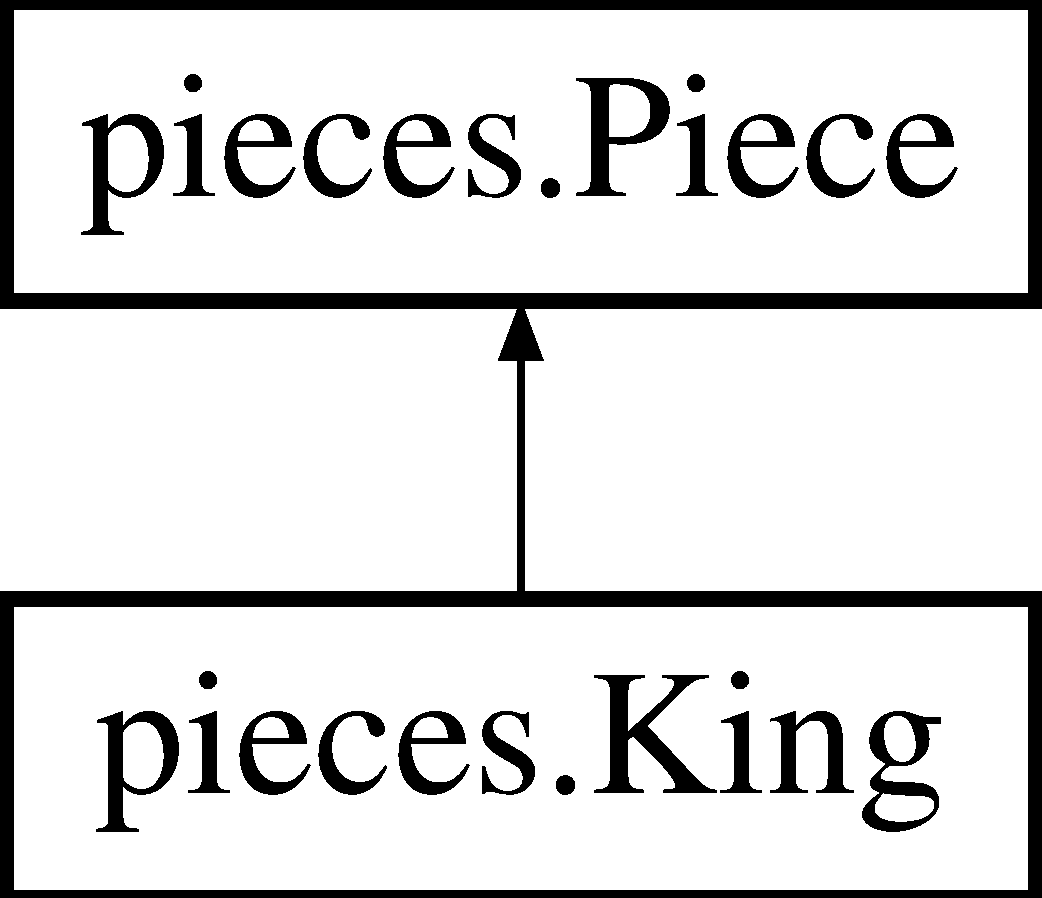
\includegraphics[height=2.000000cm]{classpieces_1_1_king}
\end{center}
\end{figure}
\subsection*{Public Member Functions}
\begin{DoxyCompactItemize}
\item 
void \hyperlink{classpieces_1_1_king_a7bfa15e882d90fbc6c5ec02f2d2dab20}{update\-Moves} (\hyperlink{classpieces_1_1_piece}{Piece}\mbox{[}$\,$\mbox{]}\mbox{[}$\,$\mbox{]} spaces, int rank, int file)
\end{DoxyCompactItemize}
\subsection*{Additional Inherited Members}


\subsection{Detailed Description}
\begin{DoxyAuthor}{Author}
Will 
\end{DoxyAuthor}


\subsection{Member Function Documentation}
\hypertarget{classpieces_1_1_king_a7bfa15e882d90fbc6c5ec02f2d2dab20}{\index{pieces\-::\-King@{pieces\-::\-King}!update\-Moves@{update\-Moves}}
\index{update\-Moves@{update\-Moves}!pieces::King@{pieces\-::\-King}}
\subsubsection[{update\-Moves}]{\setlength{\rightskip}{0pt plus 5cm}void pieces.\-King.\-update\-Moves (
\begin{DoxyParamCaption}
\item[{{\bf Piece}}]{spaces\mbox{[}$\,$\mbox{]}\mbox{[}$\,$\mbox{]}, }
\item[{int}]{rank, }
\item[{int}]{file}
\end{DoxyParamCaption}
)}}\label{classpieces_1_1_king_a7bfa15e882d90fbc6c5ec02f2d2dab20}
Updates the possible moves for the piece. Kings can move one space in any direction. 
\begin{DoxyParams}{Parameters}
{\em spaces} & the current board state \\
\hline
{\em rank} & the x (rank) location of the piece \\
\hline
{\em file} & the y (file) location of the piece \\
\hline
\end{DoxyParams}


The documentation for this class was generated from the following file\-:\begin{DoxyCompactItemize}
\item 
src/pieces/King.\-java\end{DoxyCompactItemize}

\hypertarget{classtests_1_1_king_test}{\section{tests.\-King\-Test Class Reference}
\label{classtests_1_1_king_test}\index{tests.\-King\-Test@{tests.\-King\-Test}}
}
\subsection*{Public Member Functions}
\begin{DoxyCompactItemize}
\item 
\hypertarget{classtests_1_1_king_test_aa5d2774b1e0ca4d11420ab13fdc3884c}{void {\bfseries set\-Up} ()  throws Exception }\label{classtests_1_1_king_test_aa5d2774b1e0ca4d11420ab13fdc3884c}

\item 
\hypertarget{classtests_1_1_king_test_a33d47bb640f4df0c2f3c3775dddc705e}{void {\bfseries move\-Vertical} ()}\label{classtests_1_1_king_test_a33d47bb640f4df0c2f3c3775dddc705e}

\item 
\hypertarget{classtests_1_1_king_test_ad1743fed552259c9958bc8b4dff3ec5c}{void {\bfseries move\-Horizontal} ()}\label{classtests_1_1_king_test_ad1743fed552259c9958bc8b4dff3ec5c}

\item 
\hypertarget{classtests_1_1_king_test_a52129f2b5707a86b67d2871b9e880d1a}{void {\bfseries move\-Diagonal} ()}\label{classtests_1_1_king_test_a52129f2b5707a86b67d2871b9e880d1a}

\item 
\hypertarget{classtests_1_1_king_test_acae8a279597c67995ba8b6e7434349f6}{void {\bfseries move\-More\-Spaces} ()}\label{classtests_1_1_king_test_acae8a279597c67995ba8b6e7434349f6}

\item 
\hypertarget{classtests_1_1_king_test_a461c3f492e60f53159e9070dece2c6af}{void {\bfseries capture\-Friendly} ()}\label{classtests_1_1_king_test_a461c3f492e60f53159e9070dece2c6af}

\item 
\hypertarget{classtests_1_1_king_test_adfb0cdf049dcf84bb9518412b34029af}{void {\bfseries capture\-Enemy} ()}\label{classtests_1_1_king_test_adfb0cdf049dcf84bb9518412b34029af}

\end{DoxyCompactItemize}


The documentation for this class was generated from the following file\-:\begin{DoxyCompactItemize}
\item 
src/tests/King\-Test.\-java\end{DoxyCompactItemize}

\hypertarget{classpieces_1_1_knight}{\section{pieces.\-Knight Class Reference}
\label{classpieces_1_1_knight}\index{pieces.\-Knight@{pieces.\-Knight}}
}
Inheritance diagram for pieces.\-Knight\-:\begin{figure}[H]
\begin{center}
\leavevmode
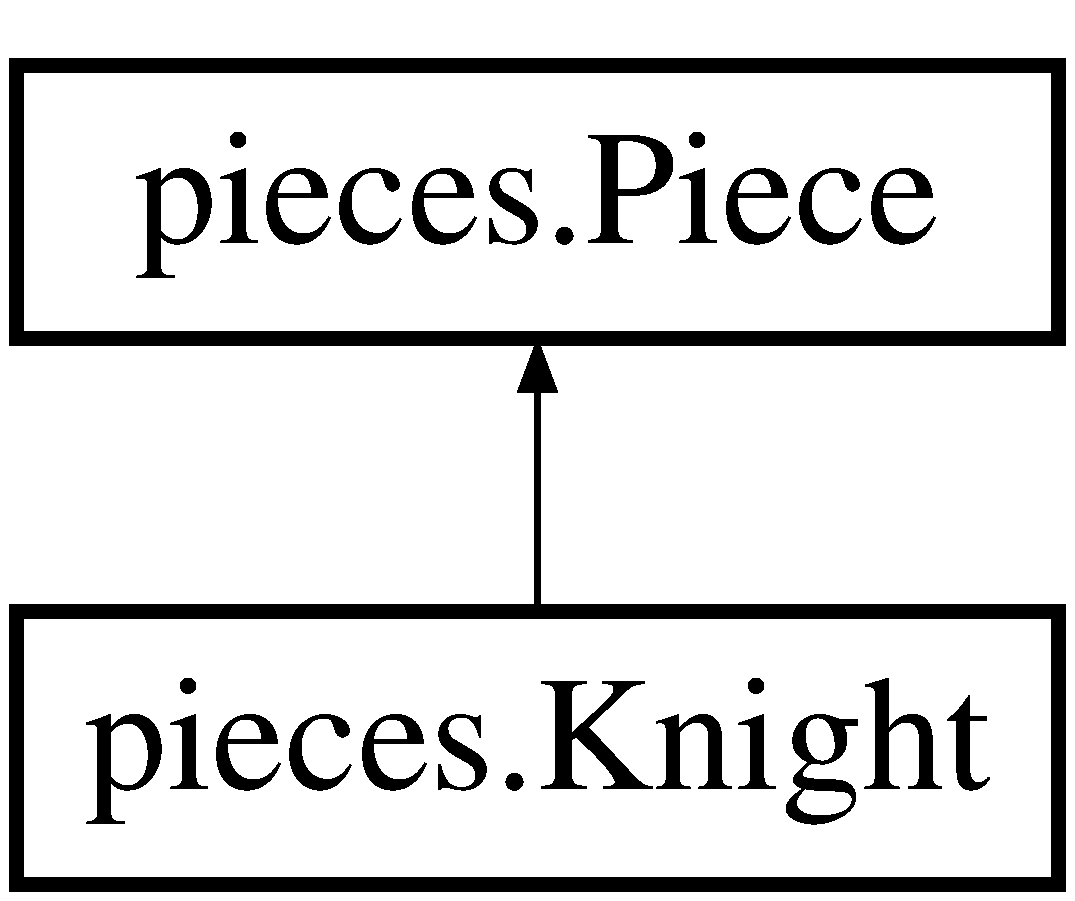
\includegraphics[height=2.000000cm]{classpieces_1_1_knight}
\end{center}
\end{figure}
\subsection*{Public Member Functions}
\begin{DoxyCompactItemize}
\item 
void \hyperlink{classpieces_1_1_knight_a6d689702e1d14b61804c2c00b2124bc9}{update\-Moves} (\hyperlink{classpieces_1_1_piece}{Piece}\mbox{[}$\,$\mbox{]}\mbox{[}$\,$\mbox{]} spaces, int rank, int file)
\end{DoxyCompactItemize}
\subsection*{Additional Inherited Members}


\subsection{Detailed Description}
\begin{DoxyAuthor}{Author}
Will 
\end{DoxyAuthor}


\subsection{Member Function Documentation}
\hypertarget{classpieces_1_1_knight_a6d689702e1d14b61804c2c00b2124bc9}{\index{pieces\-::\-Knight@{pieces\-::\-Knight}!update\-Moves@{update\-Moves}}
\index{update\-Moves@{update\-Moves}!pieces::Knight@{pieces\-::\-Knight}}
\subsubsection[{update\-Moves}]{\setlength{\rightskip}{0pt plus 5cm}void pieces.\-Knight.\-update\-Moves (
\begin{DoxyParamCaption}
\item[{{\bf Piece}}]{spaces\mbox{[}$\,$\mbox{]}\mbox{[}$\,$\mbox{]}, }
\item[{int}]{rank, }
\item[{int}]{file}
\end{DoxyParamCaption}
)}}\label{classpieces_1_1_knight_a6d689702e1d14b61804c2c00b2124bc9}
Updates the possible moves for the piece. Knights can move in L-\/shapes (combinations of 2 in one direction and 1 in another). 
\begin{DoxyParams}{Parameters}
{\em spaces} & the current board state \\
\hline
{\em rank} & the x (rank) location of the piece \\
\hline
{\em file} & the y (file) location of the piece \\
\hline
\end{DoxyParams}


The documentation for this class was generated from the following file\-:\begin{DoxyCompactItemize}
\item 
src/pieces/Knight.\-java\end{DoxyCompactItemize}

\hypertarget{classtests_1_1_knight_test}{\section{tests.\-Knight\-Test Class Reference}
\label{classtests_1_1_knight_test}\index{tests.\-Knight\-Test@{tests.\-Knight\-Test}}
}
\subsection*{Public Member Functions}
\begin{DoxyCompactItemize}
\item 
\hypertarget{classtests_1_1_knight_test_afc21f6bb2c50898bf3c3d3ae77344752}{void {\bfseries set\-Up} ()  throws Exception }\label{classtests_1_1_knight_test_afc21f6bb2c50898bf3c3d3ae77344752}

\item 
\hypertarget{classtests_1_1_knight_test_aae56788f63bdbcca2160db0ffa8ac345}{void {\bfseries knight\-Move} ()}\label{classtests_1_1_knight_test_aae56788f63bdbcca2160db0ffa8ac345}

\item 
\hypertarget{classtests_1_1_knight_test_a1cbbc10578f816892e1db40232a5c593}{void {\bfseries horizontal\-Move} ()}\label{classtests_1_1_knight_test_a1cbbc10578f816892e1db40232a5c593}

\item 
\hypertarget{classtests_1_1_knight_test_a2293f0c1c89e22b816231f573f9eff7c}{void {\bfseries vertical\-Move} ()}\label{classtests_1_1_knight_test_a2293f0c1c89e22b816231f573f9eff7c}

\item 
\hypertarget{classtests_1_1_knight_test_a9351a4b7fed2ecc5ad1a0a287a7b5366}{void {\bfseries diagonal\-Move} ()}\label{classtests_1_1_knight_test_a9351a4b7fed2ecc5ad1a0a287a7b5366}

\item 
\hypertarget{classtests_1_1_knight_test_ac90e59b248330794de2a8bd50152f7b5}{void {\bfseries capture\-Friendly} ()}\label{classtests_1_1_knight_test_ac90e59b248330794de2a8bd50152f7b5}

\item 
\hypertarget{classtests_1_1_knight_test_a5baa0f40f216230185e5c18beef82787}{void {\bfseries capture\-Opponent} ()}\label{classtests_1_1_knight_test_a5baa0f40f216230185e5c18beef82787}

\item 
\hypertarget{classtests_1_1_knight_test_a8eef748c954d221c16b0fca97ca2aeb6}{void {\bfseries jump\-Friendly} ()}\label{classtests_1_1_knight_test_a8eef748c954d221c16b0fca97ca2aeb6}

\item 
\hypertarget{classtests_1_1_knight_test_abe8f7e250d917d8b3e898e48e0cada72}{void {\bfseries jump\-Opponent} ()}\label{classtests_1_1_knight_test_abe8f7e250d917d8b3e898e48e0cada72}

\end{DoxyCompactItemize}


The documentation for this class was generated from the following file\-:\begin{DoxyCompactItemize}
\item 
src/tests/Knight\-Test.\-java\end{DoxyCompactItemize}

\hypertarget{classpieces_1_1_pawn}{\section{pieces.\-Pawn Class Reference}
\label{classpieces_1_1_pawn}\index{pieces.\-Pawn@{pieces.\-Pawn}}
}
Inheritance diagram for pieces.\-Pawn\-:\begin{figure}[H]
\begin{center}
\leavevmode
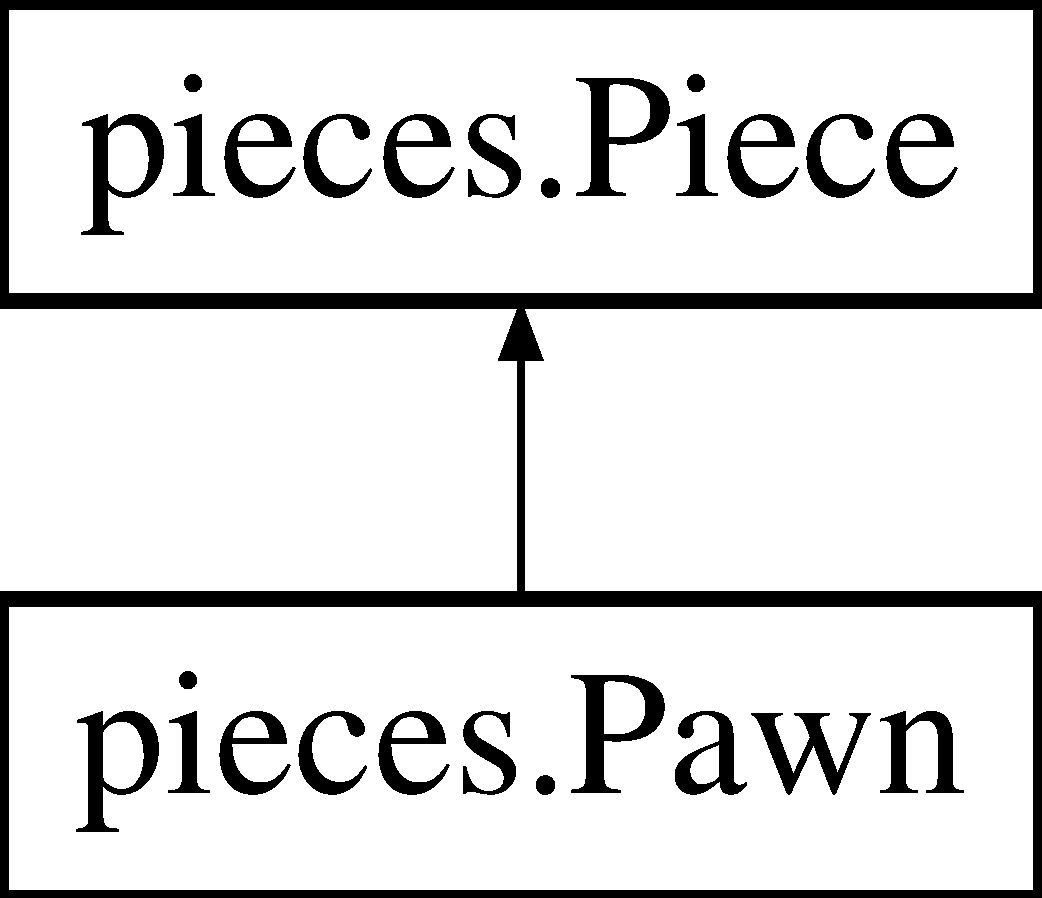
\includegraphics[height=2.000000cm]{classpieces_1_1_pawn}
\end{center}
\end{figure}
\subsection*{Public Member Functions}
\begin{DoxyCompactItemize}
\item 
void \hyperlink{classpieces_1_1_pawn_ad171a4c5739fb3ca9c5832d3252679b0}{update\-Moves} (\hyperlink{classpieces_1_1_piece}{Piece}\mbox{[}$\,$\mbox{]}\mbox{[}$\,$\mbox{]} spaces, int rank, int file)
\end{DoxyCompactItemize}
\subsection*{Additional Inherited Members}


\subsection{Detailed Description}
\begin{DoxyAuthor}{Author}
Will 
\end{DoxyAuthor}


\subsection{Member Function Documentation}
\hypertarget{classpieces_1_1_pawn_ad171a4c5739fb3ca9c5832d3252679b0}{\index{pieces\-::\-Pawn@{pieces\-::\-Pawn}!update\-Moves@{update\-Moves}}
\index{update\-Moves@{update\-Moves}!pieces::Pawn@{pieces\-::\-Pawn}}
\subsubsection[{update\-Moves}]{\setlength{\rightskip}{0pt plus 5cm}void pieces.\-Pawn.\-update\-Moves (
\begin{DoxyParamCaption}
\item[{{\bf Piece}}]{spaces\mbox{[}$\,$\mbox{]}\mbox{[}$\,$\mbox{]}, }
\item[{int}]{rank, }
\item[{int}]{file}
\end{DoxyParamCaption}
)}}\label{classpieces_1_1_pawn_ad171a4c5739fb3ca9c5832d3252679b0}
Updates the possible moves for the piece. Pawns can only move forward, and can only capture diagonally. 
\begin{DoxyParams}{Parameters}
{\em spaces} & the current board state \\
\hline
{\em rank} & the x (rank) location of the piece \\
\hline
{\em file} & the y (file) location of the piece \\
\hline
\end{DoxyParams}


The documentation for this class was generated from the following file\-:\begin{DoxyCompactItemize}
\item 
src/pieces/Pawn.\-java\end{DoxyCompactItemize}

\hypertarget{classtests_1_1_pawn_test}{\section{tests.\-Pawn\-Test Class Reference}
\label{classtests_1_1_pawn_test}\index{tests.\-Pawn\-Test@{tests.\-Pawn\-Test}}
}
\subsection*{Public Member Functions}
\begin{DoxyCompactItemize}
\item 
\hypertarget{classtests_1_1_pawn_test_a1c95ca15c50c6d846a5ca577defdb7ab}{void {\bfseries set\-Up} ()  throws Exception }\label{classtests_1_1_pawn_test_a1c95ca15c50c6d846a5ca577defdb7ab}

\item 
\hypertarget{classtests_1_1_pawn_test_a9a099bfdaa7fc6661b0112efc5dca8a3}{void {\bfseries first\-Move\-Two\-Squares} ()}\label{classtests_1_1_pawn_test_a9a099bfdaa7fc6661b0112efc5dca8a3}

\item 
\hypertarget{classtests_1_1_pawn_test_a8e62a52928e629035f0deb8b412a7dc7}{void {\bfseries double\-Special\-Move} ()}\label{classtests_1_1_pawn_test_a8e62a52928e629035f0deb8b412a7dc7}

\item 
\hypertarget{classtests_1_1_pawn_test_a263f5b34b7171296138a813bac851aba}{void {\bfseries move\-Backwards} ()}\label{classtests_1_1_pawn_test_a263f5b34b7171296138a813bac851aba}

\item 
\hypertarget{classtests_1_1_pawn_test_a9cc7c43ddffb2354f8233c3b0d536551}{void {\bfseries move\-Horizontal} ()}\label{classtests_1_1_pawn_test_a9cc7c43ddffb2354f8233c3b0d536551}

\item 
\hypertarget{classtests_1_1_pawn_test_a77c5b54ebf6f8c9e7e0aecced443981f}{void {\bfseries move\-Diagonal} ()}\label{classtests_1_1_pawn_test_a77c5b54ebf6f8c9e7e0aecced443981f}

\item 
\hypertarget{classtests_1_1_pawn_test_a2b55d34f3ffc9091f1d62818e28b5042}{void {\bfseries capture\-Backwards} ()}\label{classtests_1_1_pawn_test_a2b55d34f3ffc9091f1d62818e28b5042}

\item 
\hypertarget{classtests_1_1_pawn_test_a6cfd93a32fd5a6479c6ac43c64ee5788}{void {\bfseries capture\-Forwards} ()}\label{classtests_1_1_pawn_test_a6cfd93a32fd5a6479c6ac43c64ee5788}

\end{DoxyCompactItemize}


The documentation for this class was generated from the following file\-:\begin{DoxyCompactItemize}
\item 
src/tests/Pawn\-Test.\-java\end{DoxyCompactItemize}

\hypertarget{classpieces_1_1_piece}{\section{pieces.\-Piece Class Reference}
\label{classpieces_1_1_piece}\index{pieces.\-Piece@{pieces.\-Piece}}
}
Inheritance diagram for pieces.\-Piece\-:\begin{figure}[H]
\begin{center}
\leavevmode
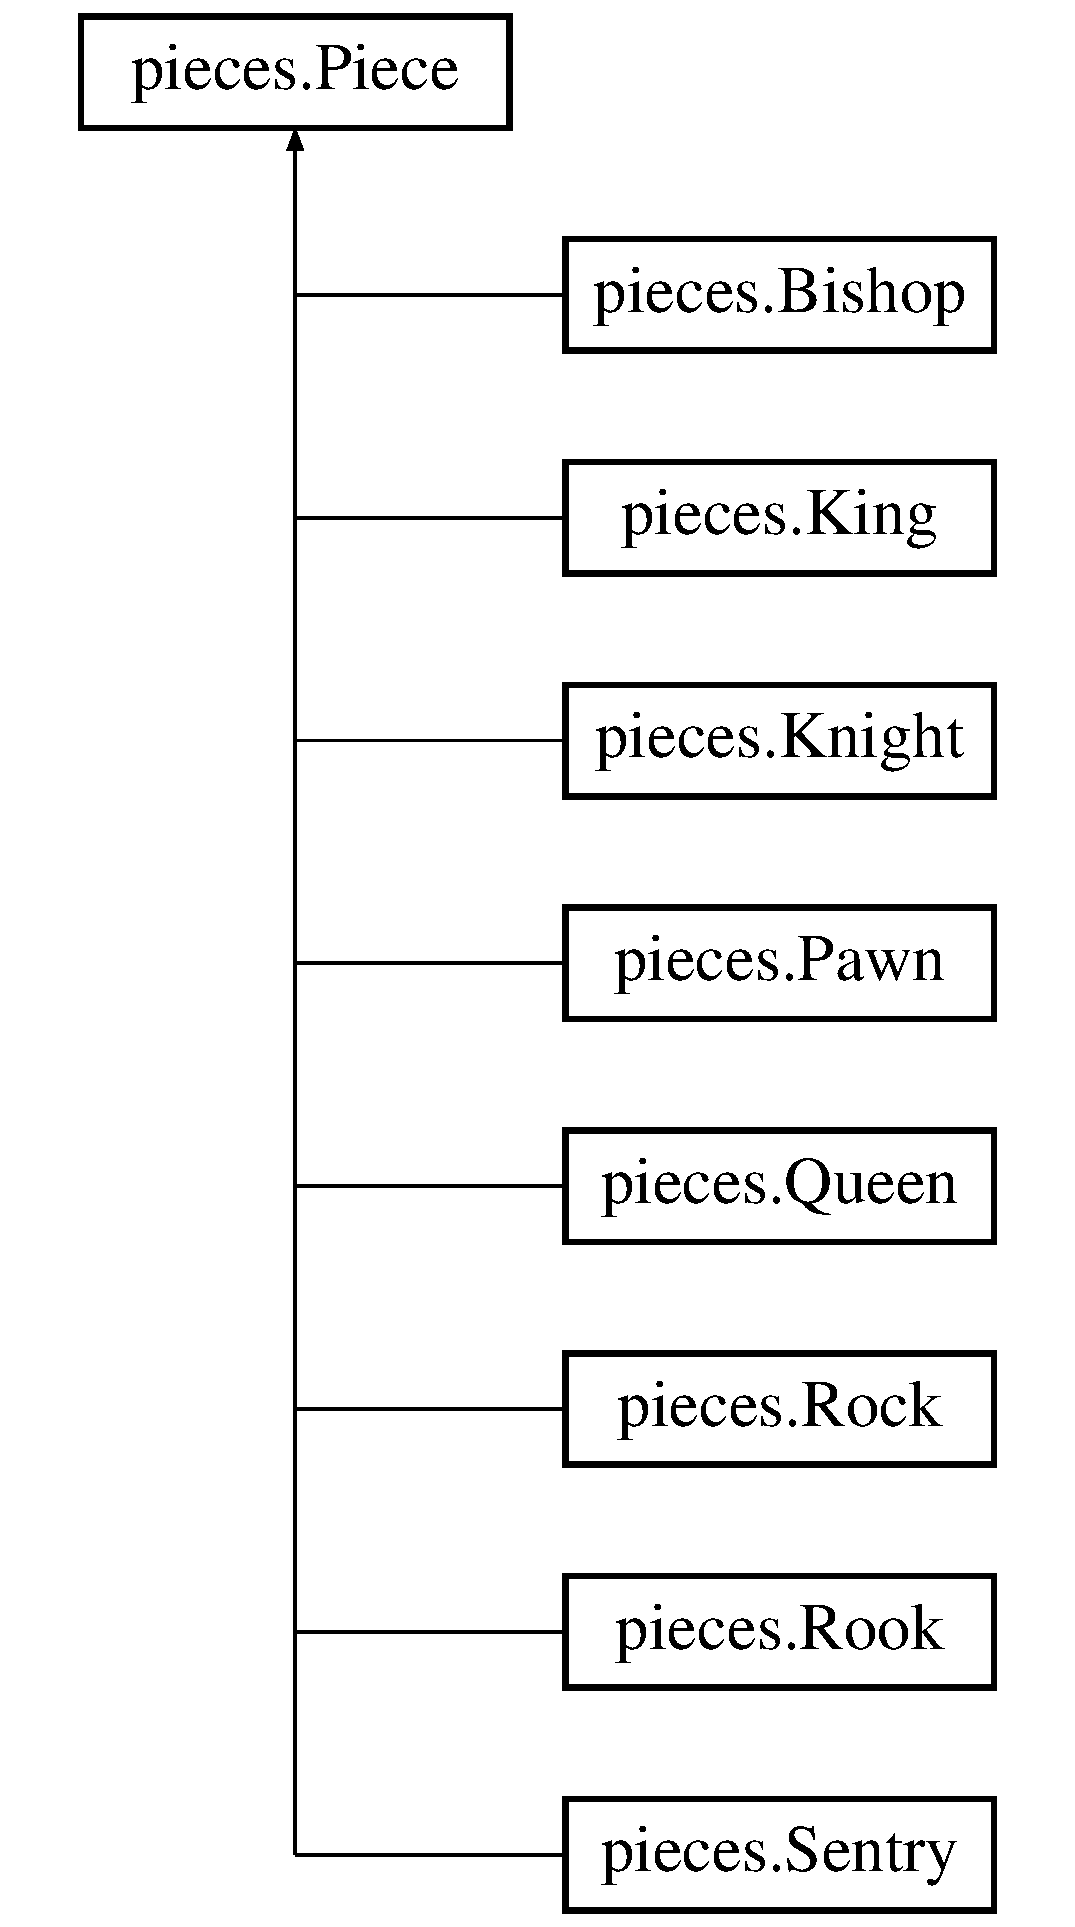
\includegraphics[height=9.000000cm]{classpieces_1_1_piece}
\end{center}
\end{figure}
\subsection*{Public Member Functions}
\begin{DoxyCompactItemize}
\item 
abstract void \hyperlink{classpieces_1_1_piece_aa05f11005bbd1b4794ec97cb9911f75a}{update\-Moves} (\hyperlink{classpieces_1_1_piece}{Piece}\mbox{[}$\,$\mbox{]}\mbox{[}$\,$\mbox{]} spaces, int rank, int file)
\item 
boolean \hyperlink{classpieces_1_1_piece_ab940424e2a0c19febbe4bb49e837a401}{is\-Valid\-Move} (\hyperlink{classmodel_1_1_space}{Space} target)
\item 
Color \hyperlink{classpieces_1_1_piece_aee0fc5fa7074b129aaf1f350ac8a7f1b}{get\-Color} ()
\item 
boolean \hyperlink{classpieces_1_1_piece_a4293bd05eab0d665a320f0bee86b498c}{same\-Owner} (\hyperlink{classpieces_1_1_piece}{Piece} other)
\item 
boolean \hyperlink{classpieces_1_1_piece_a8978c74c41b709a09b0219bf73b8a76e}{same\-Owner} (Color player)
\item 
Buffered\-Image \hyperlink{classpieces_1_1_piece_ab4468311fa6d726bcb6306ee9c350c9e}{get\-Piece\-Image} ()
\item 
boolean \hyperlink{classpieces_1_1_piece_a574e624026a0ce3f017374de87fb3ada}{can\-Capture} (\hyperlink{classmodel_1_1_space}{Space} other)
\item 
Vector$<$ \hyperlink{classmodel_1_1_space}{Space} $>$ \hyperlink{classpieces_1_1_piece_a1d7eae0ffb67821c6df54ac6adeaf5de}{get\-Moves} ()
\end{DoxyCompactItemize}
\subsection*{Static Public Member Functions}
\begin{DoxyCompactItemize}
\item 
static \hyperlink{classpieces_1_1_piece}{Piece} \hyperlink{classpieces_1_1_piece_ae4d129f2285197d6c75dbd21005ce412}{string\-To\-Piece} (String piece, Color player)
\item 
static boolean \hyperlink{classpieces_1_1_piece_a3bb514a9da872d7c44165835fa3ce4b0}{out\-Of\-Bounds} (\hyperlink{classpieces_1_1_piece}{Piece}\mbox{[}$\,$\mbox{]}\mbox{[}$\,$\mbox{]} spaces, int rank, int file)
\end{DoxyCompactItemize}
\subsection*{Protected Member Functions}
\begin{DoxyCompactItemize}
\item 
void \hyperlink{classpieces_1_1_piece_a87ecc007e69c3d6ed89a5ed34c16ebaf}{set\-Color} (Color player)
\item 
boolean \hyperlink{classpieces_1_1_piece_a92b7dd91bd1d1f79d10203123d77c071}{add\-Move} (\hyperlink{classpieces_1_1_piece}{Piece} cur\-Space, int rank, int file)
\item 
void \hyperlink{classpieces_1_1_piece_a23b77741794ea328c50796e3dcd5e360}{set\-Moves} (Vector$<$ \hyperlink{classmodel_1_1_space}{Space} $>$ \hyperlink{classpieces_1_1_piece_a64fbd75313e761ca2f13e3e542a06ec7}{moves})
\end{DoxyCompactItemize}
\subsection*{Protected Attributes}
\begin{DoxyCompactItemize}
\item 
Color \hyperlink{classpieces_1_1_piece_aad2c2ef830902ae3d7da9709976216d6}{color} = null
\item 
Vector$<$ \hyperlink{classmodel_1_1_space}{Space} $>$ \hyperlink{classpieces_1_1_piece_a64fbd75313e761ca2f13e3e542a06ec7}{moves} = null
\end{DoxyCompactItemize}


\subsection{Detailed Description}
\begin{DoxyAuthor}{Author}
Will 
\end{DoxyAuthor}


\subsection{Member Function Documentation}
\hypertarget{classpieces_1_1_piece_a92b7dd91bd1d1f79d10203123d77c071}{\index{pieces\-::\-Piece@{pieces\-::\-Piece}!add\-Move@{add\-Move}}
\index{add\-Move@{add\-Move}!pieces::Piece@{pieces\-::\-Piece}}
\subsubsection[{add\-Move}]{\setlength{\rightskip}{0pt plus 5cm}boolean pieces.\-Piece.\-add\-Move (
\begin{DoxyParamCaption}
\item[{{\bf Piece}}]{cur\-Space, }
\item[{int}]{rank, }
\item[{int}]{file}
\end{DoxyParamCaption}
)\hspace{0.3cm}{\ttfamily [protected]}}}\label{classpieces_1_1_piece_a92b7dd91bd1d1f79d10203123d77c071}
Update\-Moves helper that checks if a given square should be added. It must not have the same owner or \begin{DoxyReturn}{Returns}
true if the piece cannot jump past the square 
\end{DoxyReturn}
\hypertarget{classpieces_1_1_piece_a574e624026a0ce3f017374de87fb3ada}{\index{pieces\-::\-Piece@{pieces\-::\-Piece}!can\-Capture@{can\-Capture}}
\index{can\-Capture@{can\-Capture}!pieces::Piece@{pieces\-::\-Piece}}
\subsubsection[{can\-Capture}]{\setlength{\rightskip}{0pt plus 5cm}boolean pieces.\-Piece.\-can\-Capture (
\begin{DoxyParamCaption}
\item[{{\bf Space}}]{other}
\end{DoxyParamCaption}
)}}\label{classpieces_1_1_piece_a574e624026a0ce3f017374de87fb3ada}

\begin{DoxyParams}{Parameters}
{\em other} & the space (rank,file) to check if a piece can capture to \\
\hline
\end{DoxyParams}
\begin{DoxyReturn}{Returns}
true if a piece can capture to a space 
\end{DoxyReturn}
\hypertarget{classpieces_1_1_piece_aee0fc5fa7074b129aaf1f350ac8a7f1b}{\index{pieces\-::\-Piece@{pieces\-::\-Piece}!get\-Color@{get\-Color}}
\index{get\-Color@{get\-Color}!pieces::Piece@{pieces\-::\-Piece}}
\subsubsection[{get\-Color}]{\setlength{\rightskip}{0pt plus 5cm}Color pieces.\-Piece.\-get\-Color (
\begin{DoxyParamCaption}
{}
\end{DoxyParamCaption}
)}}\label{classpieces_1_1_piece_aee0fc5fa7074b129aaf1f350ac8a7f1b}
\begin{DoxyReturn}{Returns}
(W\-H\-I\-T\-E,B\-L\-A\-C\-K,or N\-U\-L\-L) the color of a piece 
\end{DoxyReturn}
\hypertarget{classpieces_1_1_piece_a1d7eae0ffb67821c6df54ac6adeaf5de}{\index{pieces\-::\-Piece@{pieces\-::\-Piece}!get\-Moves@{get\-Moves}}
\index{get\-Moves@{get\-Moves}!pieces::Piece@{pieces\-::\-Piece}}
\subsubsection[{get\-Moves}]{\setlength{\rightskip}{0pt plus 5cm}Vector$<${\bf Space}$>$ pieces.\-Piece.\-get\-Moves (
\begin{DoxyParamCaption}
{}
\end{DoxyParamCaption}
)}}\label{classpieces_1_1_piece_a1d7eae0ffb67821c6df54ac6adeaf5de}
\begin{DoxyReturn}{Returns}
the moves for a piece 
\end{DoxyReturn}
\hypertarget{classpieces_1_1_piece_ab4468311fa6d726bcb6306ee9c350c9e}{\index{pieces\-::\-Piece@{pieces\-::\-Piece}!get\-Piece\-Image@{get\-Piece\-Image}}
\index{get\-Piece\-Image@{get\-Piece\-Image}!pieces::Piece@{pieces\-::\-Piece}}
\subsubsection[{get\-Piece\-Image}]{\setlength{\rightskip}{0pt plus 5cm}Buffered\-Image pieces.\-Piece.\-get\-Piece\-Image (
\begin{DoxyParamCaption}
{}
\end{DoxyParamCaption}
)}}\label{classpieces_1_1_piece_ab4468311fa6d726bcb6306ee9c350c9e}
\begin{DoxyReturn}{Returns}
the image file on disk representing the piece 
\end{DoxyReturn}
\hypertarget{classpieces_1_1_piece_ab940424e2a0c19febbe4bb49e837a401}{\index{pieces\-::\-Piece@{pieces\-::\-Piece}!is\-Valid\-Move@{is\-Valid\-Move}}
\index{is\-Valid\-Move@{is\-Valid\-Move}!pieces::Piece@{pieces\-::\-Piece}}
\subsubsection[{is\-Valid\-Move}]{\setlength{\rightskip}{0pt plus 5cm}boolean pieces.\-Piece.\-is\-Valid\-Move (
\begin{DoxyParamCaption}
\item[{{\bf Space}}]{target}
\end{DoxyParamCaption}
)}}\label{classpieces_1_1_piece_ab940424e2a0c19febbe4bb49e837a401}

\begin{DoxyParams}{Parameters}
{\em target} & the (rank,file) pair on the board to move to \\
\hline
\end{DoxyParams}
\begin{DoxyReturn}{Returns}
true if a given move is possible for a piece 
\end{DoxyReturn}
\hypertarget{classpieces_1_1_piece_a3bb514a9da872d7c44165835fa3ce4b0}{\index{pieces\-::\-Piece@{pieces\-::\-Piece}!out\-Of\-Bounds@{out\-Of\-Bounds}}
\index{out\-Of\-Bounds@{out\-Of\-Bounds}!pieces::Piece@{pieces\-::\-Piece}}
\subsubsection[{out\-Of\-Bounds}]{\setlength{\rightskip}{0pt plus 5cm}static boolean pieces.\-Piece.\-out\-Of\-Bounds (
\begin{DoxyParamCaption}
\item[{Piecespaces}]{\mbox{[}$\,$\mbox{]}\mbox{[}$\,$\mbox{]}, }
\item[{int}]{rank, }
\item[{int}]{file}
\end{DoxyParamCaption}
)\hspace{0.3cm}{\ttfamily [static]}}}\label{classpieces_1_1_piece_a3bb514a9da872d7c44165835fa3ce4b0}

\begin{DoxyParams}{Parameters}
{\em spaces} & The state of the chess board. \\
\hline
{\em rank} & the x (rank) location of the piece \\
\hline
{\em file} & the y (file) location of the piece \\
\hline
\end{DoxyParams}
\begin{DoxyReturn}{Returns}
true if a given piece is out of bounds or null 
\end{DoxyReturn}
\hypertarget{classpieces_1_1_piece_a4293bd05eab0d665a320f0bee86b498c}{\index{pieces\-::\-Piece@{pieces\-::\-Piece}!same\-Owner@{same\-Owner}}
\index{same\-Owner@{same\-Owner}!pieces::Piece@{pieces\-::\-Piece}}
\subsubsection[{same\-Owner}]{\setlength{\rightskip}{0pt plus 5cm}boolean pieces.\-Piece.\-same\-Owner (
\begin{DoxyParamCaption}
\item[{{\bf Piece}}]{other}
\end{DoxyParamCaption}
)}}\label{classpieces_1_1_piece_a4293bd05eab0d665a320f0bee86b498c}

\begin{DoxyParams}{Parameters}
{\em other} & the piece to compare the current one with \\
\hline
\end{DoxyParams}
\begin{DoxyReturn}{Returns}
true if one piece has the same owner as the other 
\end{DoxyReturn}
\hypertarget{classpieces_1_1_piece_a8978c74c41b709a09b0219bf73b8a76e}{\index{pieces\-::\-Piece@{pieces\-::\-Piece}!same\-Owner@{same\-Owner}}
\index{same\-Owner@{same\-Owner}!pieces::Piece@{pieces\-::\-Piece}}
\subsubsection[{same\-Owner}]{\setlength{\rightskip}{0pt plus 5cm}boolean pieces.\-Piece.\-same\-Owner (
\begin{DoxyParamCaption}
\item[{Color}]{player}
\end{DoxyParamCaption}
)}}\label{classpieces_1_1_piece_a8978c74c41b709a09b0219bf73b8a76e}

\begin{DoxyParams}{Parameters}
{\em player} & the color of the player to check against \\
\hline
\end{DoxyParams}
\begin{DoxyReturn}{Returns}
true if the current piece is of the same color 
\end{DoxyReturn}
\hypertarget{classpieces_1_1_piece_a87ecc007e69c3d6ed89a5ed34c16ebaf}{\index{pieces\-::\-Piece@{pieces\-::\-Piece}!set\-Color@{set\-Color}}
\index{set\-Color@{set\-Color}!pieces::Piece@{pieces\-::\-Piece}}
\subsubsection[{set\-Color}]{\setlength{\rightskip}{0pt plus 5cm}void pieces.\-Piece.\-set\-Color (
\begin{DoxyParamCaption}
\item[{Color}]{player}
\end{DoxyParamCaption}
)\hspace{0.3cm}{\ttfamily [protected]}}}\label{classpieces_1_1_piece_a87ecc007e69c3d6ed89a5ed34c16ebaf}

\begin{DoxyParams}{Parameters}
{\em player} & (W\-H\-I\-T\-E,B\-L\-A\-C\-K) the color to set the piece to \\
\hline
\end{DoxyParams}
\hypertarget{classpieces_1_1_piece_a23b77741794ea328c50796e3dcd5e360}{\index{pieces\-::\-Piece@{pieces\-::\-Piece}!set\-Moves@{set\-Moves}}
\index{set\-Moves@{set\-Moves}!pieces::Piece@{pieces\-::\-Piece}}
\subsubsection[{set\-Moves}]{\setlength{\rightskip}{0pt plus 5cm}void pieces.\-Piece.\-set\-Moves (
\begin{DoxyParamCaption}
\item[{Vector$<$ {\bf Space} $>$}]{moves}
\end{DoxyParamCaption}
)\hspace{0.3cm}{\ttfamily [protected]}}}\label{classpieces_1_1_piece_a23b77741794ea328c50796e3dcd5e360}

\begin{DoxyParams}{Parameters}
{\em moves} & the moves to set for the piece \\
\hline
\end{DoxyParams}
\hypertarget{classpieces_1_1_piece_ae4d129f2285197d6c75dbd21005ce412}{\index{pieces\-::\-Piece@{pieces\-::\-Piece}!string\-To\-Piece@{string\-To\-Piece}}
\index{string\-To\-Piece@{string\-To\-Piece}!pieces::Piece@{pieces\-::\-Piece}}
\subsubsection[{string\-To\-Piece}]{\setlength{\rightskip}{0pt plus 5cm}static {\bf Piece} pieces.\-Piece.\-string\-To\-Piece (
\begin{DoxyParamCaption}
\item[{String}]{piece, }
\item[{Color}]{player}
\end{DoxyParamCaption}
)\hspace{0.3cm}{\ttfamily [static]}}}\label{classpieces_1_1_piece_ae4d129f2285197d6c75dbd21005ce412}
Converts a string to an instance of a new piece. 
\begin{DoxyParams}{Parameters}
{\em piece} & the type of piece to instantiate \\
\hline
{\em player} & the color of piece to initialize \\
\hline
\end{DoxyParams}
\begin{DoxyReturn}{Returns}
the initialized piece matching the string input 
\end{DoxyReturn}
\hypertarget{classpieces_1_1_piece_aa05f11005bbd1b4794ec97cb9911f75a}{\index{pieces\-::\-Piece@{pieces\-::\-Piece}!update\-Moves@{update\-Moves}}
\index{update\-Moves@{update\-Moves}!pieces::Piece@{pieces\-::\-Piece}}
\subsubsection[{update\-Moves}]{\setlength{\rightskip}{0pt plus 5cm}abstract void pieces.\-Piece.\-update\-Moves (
\begin{DoxyParamCaption}
\item[{{\bf Piece}}]{spaces\mbox{[}$\,$\mbox{]}\mbox{[}$\,$\mbox{]}, }
\item[{int}]{rank, }
\item[{int}]{file}
\end{DoxyParamCaption}
)\hspace{0.3cm}{\ttfamily [abstract]}}}\label{classpieces_1_1_piece_aa05f11005bbd1b4794ec97cb9911f75a}
Upates the possible moves for a given piece. 
\begin{DoxyParams}{Parameters}
{\em spaces} & The state of the chess board. \\
\hline
{\em rank} & the x (rank) location of the piece \\
\hline
{\em file} & the y (file) location of the piece \\
\hline
\end{DoxyParams}


\subsection{Member Data Documentation}
\hypertarget{classpieces_1_1_piece_aad2c2ef830902ae3d7da9709976216d6}{\index{pieces\-::\-Piece@{pieces\-::\-Piece}!color@{color}}
\index{color@{color}!pieces::Piece@{pieces\-::\-Piece}}
\subsubsection[{color}]{\setlength{\rightskip}{0pt plus 5cm}Color pieces.\-Piece.\-color = null\hspace{0.3cm}{\ttfamily [protected]}}}\label{classpieces_1_1_piece_aad2c2ef830902ae3d7da9709976216d6}
The color of a piece. (B\-L\-A\-C\-K,W\-H\-I\-T\-E,N\-U\-L\-L) \hypertarget{classpieces_1_1_piece_a64fbd75313e761ca2f13e3e542a06ec7}{\index{pieces\-::\-Piece@{pieces\-::\-Piece}!moves@{moves}}
\index{moves@{moves}!pieces::Piece@{pieces\-::\-Piece}}
\subsubsection[{moves}]{\setlength{\rightskip}{0pt plus 5cm}Vector$<${\bf Space}$>$ pieces.\-Piece.\-moves = null\hspace{0.3cm}{\ttfamily [protected]}}}\label{classpieces_1_1_piece_a64fbd75313e761ca2f13e3e542a06ec7}
The possible moves for a piece. 

The documentation for this class was generated from the following file\-:\begin{DoxyCompactItemize}
\item 
src/pieces/Piece.\-java\end{DoxyCompactItemize}

\hypertarget{classtests_1_1_piece_test}{\section{tests.\-Piece\-Test Class Reference}
\label{classtests_1_1_piece_test}\index{tests.\-Piece\-Test@{tests.\-Piece\-Test}}
}
\subsection*{Public Member Functions}
\begin{DoxyCompactItemize}
\item 
\hypertarget{classtests_1_1_piece_test_a1ab49aec08c05c3fc20f2640ec23a9cd}{void {\bfseries set\-Up} ()  throws Exception }\label{classtests_1_1_piece_test_a1ab49aec08c05c3fc20f2640ec23a9cd}

\item 
\hypertarget{classtests_1_1_piece_test_a972a9d2d0bb092b117d0ced56b647b5c}{void {\bfseries outof\-Bounds\-Set\-Piece} ()}\label{classtests_1_1_piece_test_a972a9d2d0bb092b117d0ced56b647b5c}

\item 
\hypertarget{classtests_1_1_piece_test_a33a87cee6944d5a2d70cf8ff95e4d717}{void {\bfseries bad\-Name\-Set\-Piece} ()}\label{classtests_1_1_piece_test_a33a87cee6944d5a2d70cf8ff95e4d717}

\item 
\hypertarget{classtests_1_1_piece_test_a28da89b79e8d8ee7b0245ee5ae0337d3}{void {\bfseries valid\-Set\-Piece} ()}\label{classtests_1_1_piece_test_a28da89b79e8d8ee7b0245ee5ae0337d3}

\item 
\hypertarget{classtests_1_1_piece_test_a4c2edac4d58c1f713e8cc0b4667f5950}{void {\bfseries double\-Set\-Piece} ()}\label{classtests_1_1_piece_test_a4c2edac4d58c1f713e8cc0b4667f5950}

\item 
\hypertarget{classtests_1_1_piece_test_aecd0ae7920e3db30e4e89dc8459ffeba}{void {\bfseries empty\-Move} ()}\label{classtests_1_1_piece_test_aecd0ae7920e3db30e4e89dc8459ffeba}

\item 
\hypertarget{classtests_1_1_piece_test_acc83a7d60ca8013ac8c4830daaa71816}{void {\bfseries bad\-Move} ()}\label{classtests_1_1_piece_test_acc83a7d60ca8013ac8c4830daaa71816}

\item 
\hypertarget{classtests_1_1_piece_test_a861c221cfe010242746505ec1941b130}{void {\bfseries empty\-Piece\-Move} ()}\label{classtests_1_1_piece_test_a861c221cfe010242746505ec1941b130}

\end{DoxyCompactItemize}


The documentation for this class was generated from the following file\-:\begin{DoxyCompactItemize}
\item 
src/tests/Piece\-Test.\-java\end{DoxyCompactItemize}

\hypertarget{classpieces_1_1_queen}{\section{pieces.\-Queen Class Reference}
\label{classpieces_1_1_queen}\index{pieces.\-Queen@{pieces.\-Queen}}
}
Inheritance diagram for pieces.\-Queen\-:\begin{figure}[H]
\begin{center}
\leavevmode
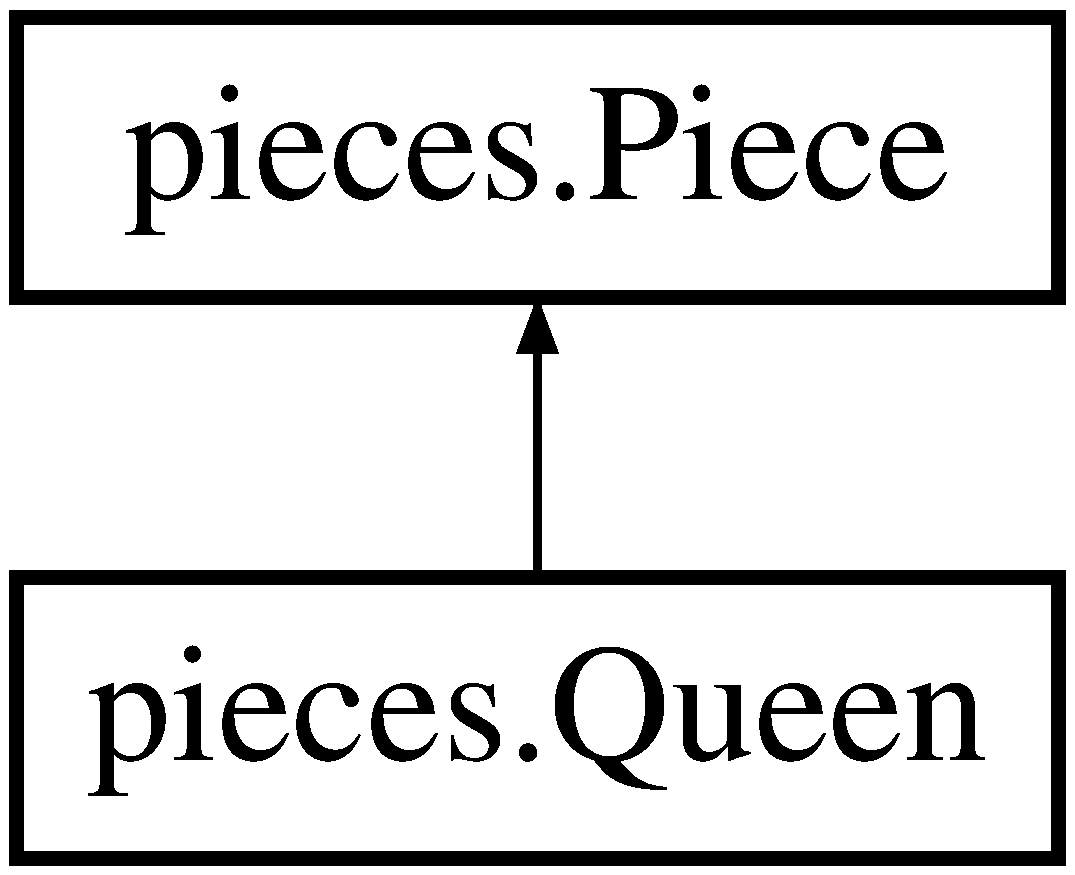
\includegraphics[height=2.000000cm]{classpieces_1_1_queen}
\end{center}
\end{figure}
\subsection*{Public Member Functions}
\begin{DoxyCompactItemize}
\item 
void \hyperlink{classpieces_1_1_queen_ab46d0c19a46b51e8d6aedddd0ef58aa7}{update\-Moves} (\hyperlink{classpieces_1_1_piece}{Piece}\mbox{[}$\,$\mbox{]}\mbox{[}$\,$\mbox{]} spaces, int rank, int file)
\end{DoxyCompactItemize}
\subsection*{Additional Inherited Members}


\subsection{Detailed Description}
\begin{DoxyAuthor}{Author}
Will 
\end{DoxyAuthor}


\subsection{Member Function Documentation}
\hypertarget{classpieces_1_1_queen_ab46d0c19a46b51e8d6aedddd0ef58aa7}{\index{pieces\-::\-Queen@{pieces\-::\-Queen}!update\-Moves@{update\-Moves}}
\index{update\-Moves@{update\-Moves}!pieces::Queen@{pieces\-::\-Queen}}
\subsubsection[{update\-Moves}]{\setlength{\rightskip}{0pt plus 5cm}void pieces.\-Queen.\-update\-Moves (
\begin{DoxyParamCaption}
\item[{{\bf Piece}}]{spaces\mbox{[}$\,$\mbox{]}\mbox{[}$\,$\mbox{]}, }
\item[{int}]{rank, }
\item[{int}]{file}
\end{DoxyParamCaption}
)}}\label{classpieces_1_1_queen_ab46d0c19a46b51e8d6aedddd0ef58aa7}
Updates the possible moves for the piece. Queens can move as many squares as possible in any direction. 
\begin{DoxyParams}{Parameters}
{\em spaces} & the current board state \\
\hline
{\em rank} & the x (rank) location of the piece \\
\hline
{\em file} & the y (file) location of the piece \\
\hline
\end{DoxyParams}


The documentation for this class was generated from the following file\-:\begin{DoxyCompactItemize}
\item 
src/pieces/Queen.\-java\end{DoxyCompactItemize}

\hypertarget{classtests_1_1_queen_test}{\section{tests.\-Queen\-Test Class Reference}
\label{classtests_1_1_queen_test}\index{tests.\-Queen\-Test@{tests.\-Queen\-Test}}
}
\subsection*{Public Member Functions}
\begin{DoxyCompactItemize}
\item 
\hypertarget{classtests_1_1_queen_test_a30352da68ac5e93587ad3d736998580c}{void {\bfseries set\-Up} ()  throws Exception }\label{classtests_1_1_queen_test_a30352da68ac5e93587ad3d736998580c}

\item 
\hypertarget{classtests_1_1_queen_test_a7e7e6d21e68c95ff16276a44b6c5383a}{void {\bfseries diagonal\-Move} ()}\label{classtests_1_1_queen_test_a7e7e6d21e68c95ff16276a44b6c5383a}

\item 
\hypertarget{classtests_1_1_queen_test_a820a919578dd44015dc6824c3809a2a0}{void {\bfseries horizontal\-Move} ()}\label{classtests_1_1_queen_test_a820a919578dd44015dc6824c3809a2a0}

\item 
\hypertarget{classtests_1_1_queen_test_ad5f5f69bf7b74c24488de4611f713b4c}{void {\bfseries vertical\-Move} ()}\label{classtests_1_1_queen_test_ad5f5f69bf7b74c24488de4611f713b4c}

\item 
\hypertarget{classtests_1_1_queen_test_aa6b17aa69ff31bc43b32aef6dc05acdf}{void {\bfseries wierd\-Move} ()}\label{classtests_1_1_queen_test_aa6b17aa69ff31bc43b32aef6dc05acdf}

\item 
\hypertarget{classtests_1_1_queen_test_a54bec46acf0e55a96af113648c58de48}{void {\bfseries capture\-Friendly} ()}\label{classtests_1_1_queen_test_a54bec46acf0e55a96af113648c58de48}

\item 
\hypertarget{classtests_1_1_queen_test_a48db6b3c45130e60612168f9f53ad7dd}{void {\bfseries capture\-Opponent} ()}\label{classtests_1_1_queen_test_a48db6b3c45130e60612168f9f53ad7dd}

\item 
\hypertarget{classtests_1_1_queen_test_a810beb7310b8db5fb539fffd208d2897}{void {\bfseries jump\-Friendly} ()}\label{classtests_1_1_queen_test_a810beb7310b8db5fb539fffd208d2897}

\item 
\hypertarget{classtests_1_1_queen_test_aa5ea3fb58576c5e42323afef4b7027c4}{void {\bfseries jump\-Enemy} ()}\label{classtests_1_1_queen_test_aa5ea3fb58576c5e42323afef4b7027c4}

\end{DoxyCompactItemize}


The documentation for this class was generated from the following file\-:\begin{DoxyCompactItemize}
\item 
src/tests/Queen\-Test.\-java\end{DoxyCompactItemize}

\hypertarget{classpieces_1_1_rock}{\section{pieces.\-Rock Class Reference}
\label{classpieces_1_1_rock}\index{pieces.\-Rock@{pieces.\-Rock}}
}
Inheritance diagram for pieces.\-Rock\-:\begin{figure}[H]
\begin{center}
\leavevmode
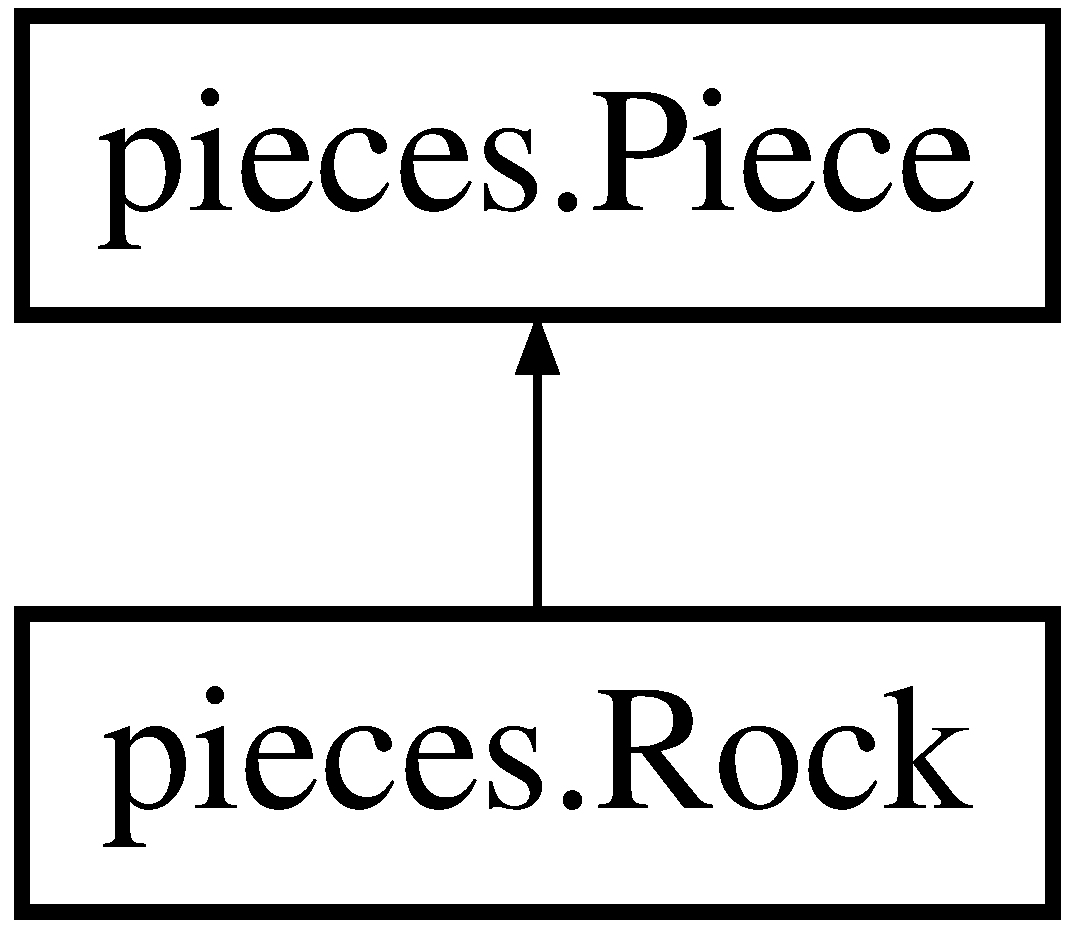
\includegraphics[height=2.000000cm]{classpieces_1_1_rock}
\end{center}
\end{figure}
\subsection*{Public Member Functions}
\begin{DoxyCompactItemize}
\item 
void \hyperlink{classpieces_1_1_rock_ae0225efa9bc90ae7a8bbe080f1ab55b6}{update\-Moves} (\hyperlink{classpieces_1_1_piece}{Piece}\mbox{[}$\,$\mbox{]}\mbox{[}$\,$\mbox{]} spaces, int rank, int file)
\end{DoxyCompactItemize}
\subsection*{Additional Inherited Members}


\subsection{Detailed Description}
\begin{DoxyAuthor}{Author}
Will 
\end{DoxyAuthor}


\subsection{Member Function Documentation}
\hypertarget{classpieces_1_1_rock_ae0225efa9bc90ae7a8bbe080f1ab55b6}{\index{pieces\-::\-Rock@{pieces\-::\-Rock}!update\-Moves@{update\-Moves}}
\index{update\-Moves@{update\-Moves}!pieces::Rock@{pieces\-::\-Rock}}
\subsubsection[{update\-Moves}]{\setlength{\rightskip}{0pt plus 5cm}void pieces.\-Rock.\-update\-Moves (
\begin{DoxyParamCaption}
\item[{{\bf Piece}}]{spaces\mbox{[}$\,$\mbox{]}\mbox{[}$\,$\mbox{]}, }
\item[{int}]{rank, }
\item[{int}]{file}
\end{DoxyParamCaption}
)}}\label{classpieces_1_1_rock_ae0225efa9bc90ae7a8bbe080f1ab55b6}
Upates the possible moves for a given piece. Rocks cannot move at all. 
\begin{DoxyParams}{Parameters}
{\em spaces} & The state of the chess board. \\
\hline
{\em rank} & the x (rank) location of the piece \\
\hline
{\em file} & the y (file) location of the piece \\
\hline
\end{DoxyParams}


The documentation for this class was generated from the following file\-:\begin{DoxyCompactItemize}
\item 
src/pieces/Rock.\-java\end{DoxyCompactItemize}

\hypertarget{classtests_1_1_rock_test}{\section{tests.\-Rock\-Test Class Reference}
\label{classtests_1_1_rock_test}\index{tests.\-Rock\-Test@{tests.\-Rock\-Test}}
}
\subsection*{Public Member Functions}
\begin{DoxyCompactItemize}
\item 
\hypertarget{classtests_1_1_rock_test_a62ac44dde9bf2da150651d6b7abad4c8}{void {\bfseries set\-Up} ()  throws Exception }\label{classtests_1_1_rock_test_a62ac44dde9bf2da150651d6b7abad4c8}

\item 
\hypertarget{classtests_1_1_rock_test_a65c8c7e1ba236c999f5108dac4bebbd8}{void {\bfseries set\-Rock} ()}\label{classtests_1_1_rock_test_a65c8c7e1ba236c999f5108dac4bebbd8}

\item 
\hypertarget{classtests_1_1_rock_test_acac906308a93a416603769d82346e20c}{void {\bfseries cant\-Move} ()}\label{classtests_1_1_rock_test_acac906308a93a416603769d82346e20c}

\end{DoxyCompactItemize}


The documentation for this class was generated from the following file\-:\begin{DoxyCompactItemize}
\item 
src/tests/Rock\-Test.\-java\end{DoxyCompactItemize}

\hypertarget{classpieces_1_1_rook}{\section{pieces.\-Rook Class Reference}
\label{classpieces_1_1_rook}\index{pieces.\-Rook@{pieces.\-Rook}}
}
Inheritance diagram for pieces.\-Rook\-:\begin{figure}[H]
\begin{center}
\leavevmode
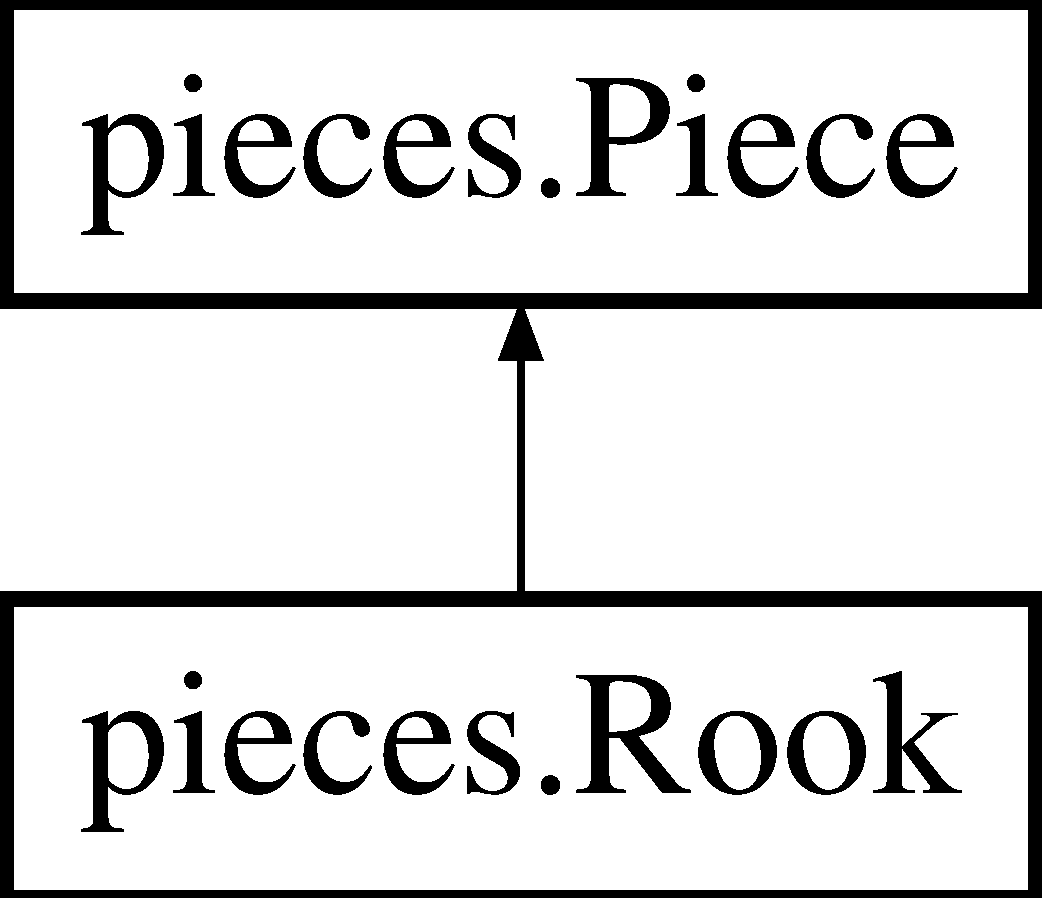
\includegraphics[height=2.000000cm]{classpieces_1_1_rook}
\end{center}
\end{figure}
\subsection*{Public Member Functions}
\begin{DoxyCompactItemize}
\item 
void \hyperlink{classpieces_1_1_rook_a4b6c88bd4942a5ff68aab59cc350152e}{update\-Moves} (\hyperlink{classpieces_1_1_piece}{Piece}\mbox{[}$\,$\mbox{]}\mbox{[}$\,$\mbox{]} spaces, int rank, int file)
\end{DoxyCompactItemize}
\subsection*{Additional Inherited Members}


\subsection{Detailed Description}
\begin{DoxyAuthor}{Author}
Will 
\end{DoxyAuthor}


\subsection{Member Function Documentation}
\hypertarget{classpieces_1_1_rook_a4b6c88bd4942a5ff68aab59cc350152e}{\index{pieces\-::\-Rook@{pieces\-::\-Rook}!update\-Moves@{update\-Moves}}
\index{update\-Moves@{update\-Moves}!pieces::Rook@{pieces\-::\-Rook}}
\subsubsection[{update\-Moves}]{\setlength{\rightskip}{0pt plus 5cm}void pieces.\-Rook.\-update\-Moves (
\begin{DoxyParamCaption}
\item[{Piecespaces}]{\mbox{[}$\,$\mbox{]}\mbox{[}$\,$\mbox{]}, }
\item[{int}]{rank, }
\item[{int}]{file}
\end{DoxyParamCaption}
)}}\label{classpieces_1_1_rook_a4b6c88bd4942a5ff68aab59cc350152e}
Upates the possible moves for a given piece. Rooks can move in straight lines horizontal and vertical. 
\begin{DoxyParams}{Parameters}
{\em spaces} & the state of the chess board. \\
\hline
{\em rank} & the x (rank) location of the piece \\
\hline
{\em file} & the y (file) location of the piece \\
\hline
\end{DoxyParams}


The documentation for this class was generated from the following file\-:\begin{DoxyCompactItemize}
\item 
src/pieces/Rook.\-java\end{DoxyCompactItemize}

\hypertarget{classtests_1_1_rook_test}{\section{tests.\-Rook\-Test Class Reference}
\label{classtests_1_1_rook_test}\index{tests.\-Rook\-Test@{tests.\-Rook\-Test}}
}
\subsection*{Public Member Functions}
\begin{DoxyCompactItemize}
\item 
\hypertarget{classtests_1_1_rook_test_ac7fe423ff8f896171b032e8880d0dacc}{void {\bfseries set\-Up} ()  throws Exception }\label{classtests_1_1_rook_test_ac7fe423ff8f896171b032e8880d0dacc}

\item 
\hypertarget{classtests_1_1_rook_test_a52e338e8983e3e1f5ed4feaa0144f2c8}{void {\bfseries rook\-Move} ()}\label{classtests_1_1_rook_test_a52e338e8983e3e1f5ed4feaa0144f2c8}

\item 
\hypertarget{classtests_1_1_rook_test_a9b6fc097864ea974cd2e0cc4ec98ac34}{void {\bfseries out\-Of\-Bounds\-Move} ()}\label{classtests_1_1_rook_test_a9b6fc097864ea974cd2e0cc4ec98ac34}

\item 
\hypertarget{classtests_1_1_rook_test_aa253359c8f3d21b225c7c53f1dadecda}{void {\bfseries diagonal\-Move} ()}\label{classtests_1_1_rook_test_aa253359c8f3d21b225c7c53f1dadecda}

\item 
\hypertarget{classtests_1_1_rook_test_aa847c3fad4c2332d76a7f2adea1d8073}{void {\bfseries weird\-Move} ()}\label{classtests_1_1_rook_test_aa847c3fad4c2332d76a7f2adea1d8073}

\item 
\hypertarget{classtests_1_1_rook_test_a7f7092edba619c12981e3b620bfa1761}{void {\bfseries capture\-Friendly} ()}\label{classtests_1_1_rook_test_a7f7092edba619c12981e3b620bfa1761}

\item 
\hypertarget{classtests_1_1_rook_test_ad6100119730fbfb1784a7ce290bace3a}{void {\bfseries capture\-Opponent} ()}\label{classtests_1_1_rook_test_ad6100119730fbfb1784a7ce290bace3a}

\item 
\hypertarget{classtests_1_1_rook_test_ac1f70f4418be047d6e3fb6911253b172}{void {\bfseries jump\-Friendly\-Pieces} ()}\label{classtests_1_1_rook_test_ac1f70f4418be047d6e3fb6911253b172}

\item 
\hypertarget{classtests_1_1_rook_test_a4c6cee3a224f404f625f6534c9ca7dfd}{void {\bfseries jump\-Enemy\-Piece} ()}\label{classtests_1_1_rook_test_a4c6cee3a224f404f625f6534c9ca7dfd}

\end{DoxyCompactItemize}


The documentation for this class was generated from the following file\-:\begin{DoxyCompactItemize}
\item 
src/tests/Rook\-Test.\-java\end{DoxyCompactItemize}

\hypertarget{classpieces_1_1_sentry}{\section{pieces.\-Sentry Class Reference}
\label{classpieces_1_1_sentry}\index{pieces.\-Sentry@{pieces.\-Sentry}}
}
Inheritance diagram for pieces.\-Sentry\-:\begin{figure}[H]
\begin{center}
\leavevmode
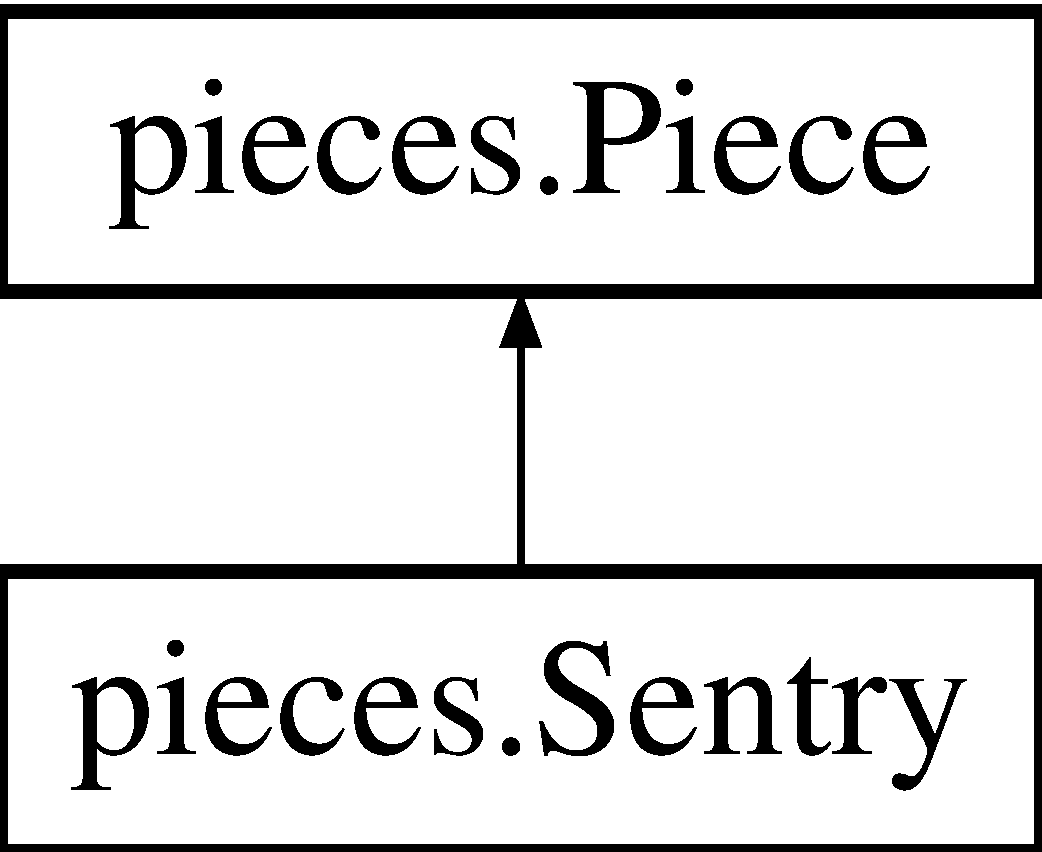
\includegraphics[height=2.000000cm]{classpieces_1_1_sentry}
\end{center}
\end{figure}
\subsection*{Public Member Functions}
\begin{DoxyCompactItemize}
\item 
void \hyperlink{classpieces_1_1_sentry_adcb012c99152748beac7471025a80ba0}{update\-Moves} (\hyperlink{classpieces_1_1_piece}{Piece}\mbox{[}$\,$\mbox{]}\mbox{[}$\,$\mbox{]} spaces, int rank, int file)
\end{DoxyCompactItemize}
\subsection*{Additional Inherited Members}


\subsection{Detailed Description}
\begin{DoxyAuthor}{Author}
Will 
\end{DoxyAuthor}


\subsection{Member Function Documentation}
\hypertarget{classpieces_1_1_sentry_adcb012c99152748beac7471025a80ba0}{\index{pieces\-::\-Sentry@{pieces\-::\-Sentry}!update\-Moves@{update\-Moves}}
\index{update\-Moves@{update\-Moves}!pieces::Sentry@{pieces\-::\-Sentry}}
\subsubsection[{update\-Moves}]{\setlength{\rightskip}{0pt plus 5cm}void pieces.\-Sentry.\-update\-Moves (
\begin{DoxyParamCaption}
\item[{{\bf Piece}}]{spaces\mbox{[}$\,$\mbox{]}\mbox{[}$\,$\mbox{]}, }
\item[{int}]{rank, }
\item[{int}]{file}
\end{DoxyParamCaption}
)}}\label{classpieces_1_1_sentry_adcb012c99152748beac7471025a80ba0}
Upates the possible moves for a given piece. Sentries can move 2 spaces in any direction. 
\begin{DoxyParams}{Parameters}
{\em spaces} & The state of the chess board. \\
\hline
{\em rank} & the x (rank) location of the piece \\
\hline
{\em file} & the y (file) location of the piece \\
\hline
\end{DoxyParams}


The documentation for this class was generated from the following file\-:\begin{DoxyCompactItemize}
\item 
src/pieces/Sentry.\-java\end{DoxyCompactItemize}

\hypertarget{classtests_1_1_sentry_test}{\section{tests.\-Sentry\-Test Class Reference}
\label{classtests_1_1_sentry_test}\index{tests.\-Sentry\-Test@{tests.\-Sentry\-Test}}
}
\subsection*{Public Member Functions}
\begin{DoxyCompactItemize}
\item 
\hypertarget{classtests_1_1_sentry_test_a346ac0b6625ac921430016f054eaf6bd}{void {\bfseries set\-Up} ()  throws Exception }\label{classtests_1_1_sentry_test_a346ac0b6625ac921430016f054eaf6bd}

\item 
\hypertarget{classtests_1_1_sentry_test_a1ee0cfe7a78434ec7b0ae297e38265c8}{void {\bfseries set\-Sentry} ()}\label{classtests_1_1_sentry_test_a1ee0cfe7a78434ec7b0ae297e38265c8}

\item 
\hypertarget{classtests_1_1_sentry_test_a7565d39a18d4eba1be91e40714a64783}{void {\bfseries wierd\-Move} ()}\label{classtests_1_1_sentry_test_a7565d39a18d4eba1be91e40714a64783}

\item 
\hypertarget{classtests_1_1_sentry_test_a905987921d6adb2893eb85f481477e22}{void {\bfseries move\-One\-Diagonal} ()}\label{classtests_1_1_sentry_test_a905987921d6adb2893eb85f481477e22}

\item 
\hypertarget{classtests_1_1_sentry_test_ae1b67f425efd2cc09a186b1798b2ea1b}{void {\bfseries move\-Two\-Diagonal} ()}\label{classtests_1_1_sentry_test_ae1b67f425efd2cc09a186b1798b2ea1b}

\item 
\hypertarget{classtests_1_1_sentry_test_ac0f0f65933d4e3e466a97fc02172eb1d}{void {\bfseries move\-One\-Horizontal} ()}\label{classtests_1_1_sentry_test_ac0f0f65933d4e3e466a97fc02172eb1d}

\item 
\hypertarget{classtests_1_1_sentry_test_a02e1db2cbb3ada5e4af6892df520237e}{void {\bfseries move\-One\-Vertical} ()}\label{classtests_1_1_sentry_test_a02e1db2cbb3ada5e4af6892df520237e}

\item 
\hypertarget{classtests_1_1_sentry_test_acee078c5bb2903480a2dd28c64ae145d}{void {\bfseries move\-Two\-Horizontal} ()}\label{classtests_1_1_sentry_test_acee078c5bb2903480a2dd28c64ae145d}

\item 
\hypertarget{classtests_1_1_sentry_test_a706c98241cf1dc4cb68643c2519c8bae}{void {\bfseries move\-Two\-Vertical} ()}\label{classtests_1_1_sentry_test_a706c98241cf1dc4cb68643c2519c8bae}

\end{DoxyCompactItemize}


The documentation for this class was generated from the following file\-:\begin{DoxyCompactItemize}
\item 
src/tests/Sentry\-Test.\-java\end{DoxyCompactItemize}

\hypertarget{classmodel_1_1_space}{\section{model.\-Space Class Reference}
\label{classmodel_1_1_space}\index{model.\-Space@{model.\-Space}}
}
\subsection*{Public Member Functions}
\begin{DoxyCompactItemize}
\item 
\hyperlink{classmodel_1_1_space_a102225bd506d830f347c5f7d24ef11b4}{Space} (int r, int f)
\item 
int \hyperlink{classmodel_1_1_space_a6f3e57c9a3794afbdd1b60e8264eda1d}{rank} ()
\item 
int \hyperlink{classmodel_1_1_space_a444e4f1f72783c2210f3281487085519}{file} ()
\item 
boolean \hyperlink{classmodel_1_1_space_a3e3cf928913dd8eb206183f17ac1dfb6}{equals} (\hyperlink{classmodel_1_1_space}{Space} other)
\end{DoxyCompactItemize}


\subsection{Detailed Description}
\begin{DoxyAuthor}{Author}
Will 
\end{DoxyAuthor}


\subsection{Constructor \& Destructor Documentation}
\hypertarget{classmodel_1_1_space_a102225bd506d830f347c5f7d24ef11b4}{\index{model\-::\-Space@{model\-::\-Space}!Space@{Space}}
\index{Space@{Space}!model::Space@{model\-::\-Space}}
\subsubsection[{Space}]{\setlength{\rightskip}{0pt plus 5cm}model.\-Space.\-Space (
\begin{DoxyParamCaption}
\item[{int}]{r, }
\item[{int}]{f}
\end{DoxyParamCaption}
)}}\label{classmodel_1_1_space_a102225bd506d830f347c5f7d24ef11b4}

\begin{DoxyParams}{Parameters}
{\em r} & the rank (x position) of a board space \\
\hline
{\em f} & the file (y position) of a board space \\
\hline
\end{DoxyParams}


\subsection{Member Function Documentation}
\hypertarget{classmodel_1_1_space_a3e3cf928913dd8eb206183f17ac1dfb6}{\index{model\-::\-Space@{model\-::\-Space}!equals@{equals}}
\index{equals@{equals}!model::Space@{model\-::\-Space}}
\subsubsection[{equals}]{\setlength{\rightskip}{0pt plus 5cm}boolean model.\-Space.\-equals (
\begin{DoxyParamCaption}
\item[{{\bf Space}}]{other}
\end{DoxyParamCaption}
)}}\label{classmodel_1_1_space_a3e3cf928913dd8eb206183f17ac1dfb6}

\begin{DoxyParams}{Parameters}
{\em other} & the other space (rank,file) to compare to \\
\hline
\end{DoxyParams}
\begin{DoxyReturn}{Returns}
true if one space the same (x,y) position of another 
\end{DoxyReturn}
\hypertarget{classmodel_1_1_space_a444e4f1f72783c2210f3281487085519}{\index{model\-::\-Space@{model\-::\-Space}!file@{file}}
\index{file@{file}!model::Space@{model\-::\-Space}}
\subsubsection[{file}]{\setlength{\rightskip}{0pt plus 5cm}int model.\-Space.\-file (
\begin{DoxyParamCaption}
{}
\end{DoxyParamCaption}
)}}\label{classmodel_1_1_space_a444e4f1f72783c2210f3281487085519}
\begin{DoxyReturn}{Returns}
the file (y position) of a given space 
\end{DoxyReturn}
\hypertarget{classmodel_1_1_space_a6f3e57c9a3794afbdd1b60e8264eda1d}{\index{model\-::\-Space@{model\-::\-Space}!rank@{rank}}
\index{rank@{rank}!model::Space@{model\-::\-Space}}
\subsubsection[{rank}]{\setlength{\rightskip}{0pt plus 5cm}int model.\-Space.\-rank (
\begin{DoxyParamCaption}
{}
\end{DoxyParamCaption}
)}}\label{classmodel_1_1_space_a6f3e57c9a3794afbdd1b60e8264eda1d}
\begin{DoxyReturn}{Returns}
the rank (x position) of a given space 
\end{DoxyReturn}


The documentation for this class was generated from the following file\-:\begin{DoxyCompactItemize}
\item 
src/model/Space.\-java\end{DoxyCompactItemize}

\hypertarget{classcontroller_1_1_spring_utilities}{\section{controller.\-Spring\-Utilities Class Reference}
\label{classcontroller_1_1_spring_utilities}\index{controller.\-Spring\-Utilities@{controller.\-Spring\-Utilities}}
}
\subsection*{Static Public Member Functions}
\begin{DoxyCompactItemize}
\item 
static void \hyperlink{classcontroller_1_1_spring_utilities_ab25bdda847d4fe39c5d63cc96c085780}{print\-Sizes} (Component c)
\item 
static void \hyperlink{classcontroller_1_1_spring_utilities_aeeff2319a4cfb70260cf61218c17546c}{make\-Grid} (Container parent, int rows, int cols, int initial\-X, int initial\-Y, int x\-Pad, int y\-Pad)
\item 
static void \hyperlink{classcontroller_1_1_spring_utilities_a151ce024b64cd12c25ef15bb200236be}{make\-Compact\-Grid} (Container parent, int rows, int cols, int initial\-X, int initial\-Y, int x\-Pad, int y\-Pad)
\end{DoxyCompactItemize}


\subsection{Detailed Description}
A 1.\-4 file that provides utility methods for creating form-\/ or grid-\/style layouts with Spring\-Layout. These utilities are used by several programs, such as Spring\-Box and Spring\-Compact\-Grid. 

\subsection{Member Function Documentation}
\hypertarget{classcontroller_1_1_spring_utilities_a151ce024b64cd12c25ef15bb200236be}{\index{controller\-::\-Spring\-Utilities@{controller\-::\-Spring\-Utilities}!make\-Compact\-Grid@{make\-Compact\-Grid}}
\index{make\-Compact\-Grid@{make\-Compact\-Grid}!controller::SpringUtilities@{controller\-::\-Spring\-Utilities}}
\subsubsection[{make\-Compact\-Grid}]{\setlength{\rightskip}{0pt plus 5cm}static void controller.\-Spring\-Utilities.\-make\-Compact\-Grid (
\begin{DoxyParamCaption}
\item[{Container}]{parent, }
\item[{int}]{rows, }
\item[{int}]{cols, }
\item[{int}]{initial\-X, }
\item[{int}]{initial\-Y, }
\item[{int}]{x\-Pad, }
\item[{int}]{y\-Pad}
\end{DoxyParamCaption}
)\hspace{0.3cm}{\ttfamily [static]}}}\label{classcontroller_1_1_spring_utilities_a151ce024b64cd12c25ef15bb200236be}
Aligns the first {\ttfamily rows} $\ast$ {\ttfamily cols} components of {\ttfamily parent} in a grid. Each component in a column is as wide as the maximum preferred width of the components in that column; height is similarly determined for each row. The parent is made just big enough to fit them all.


\begin{DoxyParams}{Parameters}
{\em rows} & number of rows \\
\hline
{\em cols} & number of columns \\
\hline
{\em initial\-X} & x location to start the grid at \\
\hline
{\em initial\-Y} & y location to start the grid at \\
\hline
{\em x\-Pad} & x padding between cells \\
\hline
{\em y\-Pad} & y padding between cells \\
\hline
\end{DoxyParams}
\hypertarget{classcontroller_1_1_spring_utilities_aeeff2319a4cfb70260cf61218c17546c}{\index{controller\-::\-Spring\-Utilities@{controller\-::\-Spring\-Utilities}!make\-Grid@{make\-Grid}}
\index{make\-Grid@{make\-Grid}!controller::SpringUtilities@{controller\-::\-Spring\-Utilities}}
\subsubsection[{make\-Grid}]{\setlength{\rightskip}{0pt plus 5cm}static void controller.\-Spring\-Utilities.\-make\-Grid (
\begin{DoxyParamCaption}
\item[{Container}]{parent, }
\item[{int}]{rows, }
\item[{int}]{cols, }
\item[{int}]{initial\-X, }
\item[{int}]{initial\-Y, }
\item[{int}]{x\-Pad, }
\item[{int}]{y\-Pad}
\end{DoxyParamCaption}
)\hspace{0.3cm}{\ttfamily [static]}}}\label{classcontroller_1_1_spring_utilities_aeeff2319a4cfb70260cf61218c17546c}
Aligns the first {\ttfamily rows} $\ast$ {\ttfamily cols} components of {\ttfamily parent} in a grid. Each component is as big as the maximum preferred width and height of the components. The parent is made just big enough to fit them all.


\begin{DoxyParams}{Parameters}
{\em rows} & number of rows \\
\hline
{\em cols} & number of columns \\
\hline
{\em initial\-X} & x location to start the grid at \\
\hline
{\em initial\-Y} & y location to start the grid at \\
\hline
{\em x\-Pad} & x padding between cells \\
\hline
{\em y\-Pad} & y padding between cells \\
\hline
\end{DoxyParams}
\hypertarget{classcontroller_1_1_spring_utilities_ab25bdda847d4fe39c5d63cc96c085780}{\index{controller\-::\-Spring\-Utilities@{controller\-::\-Spring\-Utilities}!print\-Sizes@{print\-Sizes}}
\index{print\-Sizes@{print\-Sizes}!controller::SpringUtilities@{controller\-::\-Spring\-Utilities}}
\subsubsection[{print\-Sizes}]{\setlength{\rightskip}{0pt plus 5cm}static void controller.\-Spring\-Utilities.\-print\-Sizes (
\begin{DoxyParamCaption}
\item[{Component}]{c}
\end{DoxyParamCaption}
)\hspace{0.3cm}{\ttfamily [static]}}}\label{classcontroller_1_1_spring_utilities_ab25bdda847d4fe39c5d63cc96c085780}
A debugging utility that prints to stdout the component's minimum, preferred, and maximum sizes. 

The documentation for this class was generated from the following file\-:\begin{DoxyCompactItemize}
\item 
src/controller/Spring\-Utilities.\-java\end{DoxyCompactItemize}

\hypertarget{classcontroller_1_1_text_input}{\section{controller.\-Text\-Input Class Reference}
\label{classcontroller_1_1_text_input}\index{controller.\-Text\-Input@{controller.\-Text\-Input}}
}
Inheritance diagram for controller.\-Text\-Input\-:\begin{figure}[H]
\begin{center}
\leavevmode
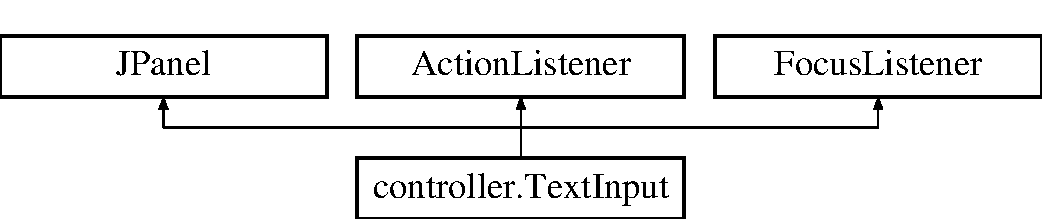
\includegraphics[height=2.000000cm]{classcontroller_1_1_text_input}
\end{center}
\end{figure}
\subsection*{Public Member Functions}
\begin{DoxyCompactItemize}
\item 
\hyperlink{classcontroller_1_1_text_input_a76a124852e34a64a21b5b74ce812ddaa}{Text\-Input} ()
\item 
void \hyperlink{classcontroller_1_1_text_input_adcac245938697e197f542f570cffd793}{action\-Performed} (Action\-Event e)
\item 
void \hyperlink{classcontroller_1_1_text_input_aacfb1f19223c451a9440dc561b17cf98}{focus\-Gained} (Focus\-Event e)
\item 
void \hyperlink{classcontroller_1_1_text_input_ad1ff76e878ea676f80232d5796f0c006}{focus\-Lost} (Focus\-Event e)
\item 
String\mbox{[}$\,$\mbox{]} \hyperlink{classcontroller_1_1_text_input_ab178b0020e8da80e7f355b8d80282e2a}{get\-Values} (int x)
\end{DoxyCompactItemize}
\subsection*{Static Public Member Functions}
\begin{DoxyCompactItemize}
\item 
static void \hyperlink{classcontroller_1_1_text_input_a5ae92539dc711f6d646808902a9a9762}{create\-And\-Show\-G\-U\-I} ()
\end{DoxyCompactItemize}
\subsection*{Protected Member Functions}
\begin{DoxyCompactItemize}
\item 
J\-Component \hyperlink{classcontroller_1_1_text_input_a4072a685676c67fe9a8d6b3b39fe95c1}{create\-Buttons} ()
\item 
Mask\-Formatter \hyperlink{classcontroller_1_1_text_input_ab347a852362f9e4796696bb3159e1649}{create\-Formatter} (String s)
\item 
void \hyperlink{classcontroller_1_1_text_input_a808ce5525f1ef4685294c487f8b0e8d4}{select\-It\-Later} (Component c)
\item 
J\-Component \hyperlink{classcontroller_1_1_text_input_a98407daf22f28cc3f219548afd455394}{create\-Entry\-Fields} ()
\end{DoxyCompactItemize}


\subsection{Detailed Description}
Text\-Input.\-java uses these additional files\-: Spring\-Utilities.\-java ... 

\subsection{Constructor \& Destructor Documentation}
\hypertarget{classcontroller_1_1_text_input_a76a124852e34a64a21b5b74ce812ddaa}{\index{controller\-::\-Text\-Input@{controller\-::\-Text\-Input}!Text\-Input@{Text\-Input}}
\index{Text\-Input@{Text\-Input}!controller::TextInput@{controller\-::\-Text\-Input}}
\subsubsection[{Text\-Input}]{\setlength{\rightskip}{0pt plus 5cm}controller.\-Text\-Input.\-Text\-Input (
\begin{DoxyParamCaption}
{}
\end{DoxyParamCaption}
)}}\label{classcontroller_1_1_text_input_a76a124852e34a64a21b5b74ce812ddaa}
Input constructor. Creates a item to add to the ending frame. Don't allow us to stretch vertically. 

\subsection{Member Function Documentation}
\hypertarget{classcontroller_1_1_text_input_adcac245938697e197f542f570cffd793}{\index{controller\-::\-Text\-Input@{controller\-::\-Text\-Input}!action\-Performed@{action\-Performed}}
\index{action\-Performed@{action\-Performed}!controller::TextInput@{controller\-::\-Text\-Input}}
\subsubsection[{action\-Performed}]{\setlength{\rightskip}{0pt plus 5cm}void controller.\-Text\-Input.\-action\-Performed (
\begin{DoxyParamCaption}
\item[{Action\-Event}]{e}
\end{DoxyParamCaption}
)}}\label{classcontroller_1_1_text_input_adcac245938697e197f542f570cffd793}
Called when the user clicks the button or presses Enter in a text field. 
\begin{DoxyParams}{Parameters}
{\em e} & the action event triggered by the user \\
\hline
\end{DoxyParams}
\hypertarget{classcontroller_1_1_text_input_a5ae92539dc711f6d646808902a9a9762}{\index{controller\-::\-Text\-Input@{controller\-::\-Text\-Input}!create\-And\-Show\-G\-U\-I@{create\-And\-Show\-G\-U\-I}}
\index{create\-And\-Show\-G\-U\-I@{create\-And\-Show\-G\-U\-I}!controller::TextInput@{controller\-::\-Text\-Input}}
\subsubsection[{create\-And\-Show\-G\-U\-I}]{\setlength{\rightskip}{0pt plus 5cm}static void controller.\-Text\-Input.\-create\-And\-Show\-G\-U\-I (
\begin{DoxyParamCaption}
{}
\end{DoxyParamCaption}
)\hspace{0.3cm}{\ttfamily [static]}}}\label{classcontroller_1_1_text_input_a5ae92539dc711f6d646808902a9a9762}
Create the G\-U\-I and show it. For thread safety, this method should be invoked from the event dispatch thread. Create and set up the window. Add contents to the window. Display the window. \hypertarget{classcontroller_1_1_text_input_a4072a685676c67fe9a8d6b3b39fe95c1}{\index{controller\-::\-Text\-Input@{controller\-::\-Text\-Input}!create\-Buttons@{create\-Buttons}}
\index{create\-Buttons@{create\-Buttons}!controller::TextInput@{controller\-::\-Text\-Input}}
\subsubsection[{create\-Buttons}]{\setlength{\rightskip}{0pt plus 5cm}J\-Component controller.\-Text\-Input.\-create\-Buttons (
\begin{DoxyParamCaption}
{}
\end{DoxyParamCaption}
)\hspace{0.3cm}{\ttfamily [protected]}}}\label{classcontroller_1_1_text_input_a4072a685676c67fe9a8d6b3b39fe95c1}
Generates the buttons for the text input prompt. Match the Spring\-Layout's gap, subtracting 5 to make up for the default gap Flow\-Layout provides. \begin{DoxyReturn}{Returns}
the new backgrond component for the text box. 
\end{DoxyReturn}
\hypertarget{classcontroller_1_1_text_input_a98407daf22f28cc3f219548afd455394}{\index{controller\-::\-Text\-Input@{controller\-::\-Text\-Input}!create\-Entry\-Fields@{create\-Entry\-Fields}}
\index{create\-Entry\-Fields@{create\-Entry\-Fields}!controller::TextInput@{controller\-::\-Text\-Input}}
\subsubsection[{create\-Entry\-Fields}]{\setlength{\rightskip}{0pt plus 5cm}J\-Component controller.\-Text\-Input.\-create\-Entry\-Fields (
\begin{DoxyParamCaption}
{}
\end{DoxyParamCaption}
)\hspace{0.3cm}{\ttfamily [protected]}}}\label{classcontroller_1_1_text_input_a98407daf22f28cc3f219548afd455394}
Associate label/field pairs, add everything, and lay it out. Add listeners to each field. \begin{DoxyReturn}{Returns}
the component containing the labels for the text input. 
\end{DoxyReturn}
\hypertarget{classcontroller_1_1_text_input_ab347a852362f9e4796696bb3159e1649}{\index{controller\-::\-Text\-Input@{controller\-::\-Text\-Input}!create\-Formatter@{create\-Formatter}}
\index{create\-Formatter@{create\-Formatter}!controller::TextInput@{controller\-::\-Text\-Input}}
\subsubsection[{create\-Formatter}]{\setlength{\rightskip}{0pt plus 5cm}Mask\-Formatter controller.\-Text\-Input.\-create\-Formatter (
\begin{DoxyParamCaption}
\item[{String}]{s}
\end{DoxyParamCaption}
)\hspace{0.3cm}{\ttfamily [protected]}}}\label{classcontroller_1_1_text_input_ab347a852362f9e4796696bb3159e1649}
A convenience method for creating a Mask\-Formatter. 
\begin{DoxyParams}{Parameters}
{\em s} & the string for creating a new formatter \\
\hline
\end{DoxyParams}
\begin{DoxyReturn}{Returns}
the resulting formatter 
\end{DoxyReturn}
\hypertarget{classcontroller_1_1_text_input_aacfb1f19223c451a9440dc561b17cf98}{\index{controller\-::\-Text\-Input@{controller\-::\-Text\-Input}!focus\-Gained@{focus\-Gained}}
\index{focus\-Gained@{focus\-Gained}!controller::TextInput@{controller\-::\-Text\-Input}}
\subsubsection[{focus\-Gained}]{\setlength{\rightskip}{0pt plus 5cm}void controller.\-Text\-Input.\-focus\-Gained (
\begin{DoxyParamCaption}
\item[{Focus\-Event}]{e}
\end{DoxyParamCaption}
)}}\label{classcontroller_1_1_text_input_aacfb1f19223c451a9440dc561b17cf98}
Called when one of the fields gets the focus so that we can select the focused field. 
\begin{DoxyParams}{Parameters}
{\em e} & an event that occurs when text is added to the input pane \\
\hline
\end{DoxyParams}
\hypertarget{classcontroller_1_1_text_input_ad1ff76e878ea676f80232d5796f0c006}{\index{controller\-::\-Text\-Input@{controller\-::\-Text\-Input}!focus\-Lost@{focus\-Lost}}
\index{focus\-Lost@{focus\-Lost}!controller::TextInput@{controller\-::\-Text\-Input}}
\subsubsection[{focus\-Lost}]{\setlength{\rightskip}{0pt plus 5cm}void controller.\-Text\-Input.\-focus\-Lost (
\begin{DoxyParamCaption}
\item[{Focus\-Event}]{e}
\end{DoxyParamCaption}
)}}\label{classcontroller_1_1_text_input_ad1ff76e878ea676f80232d5796f0c006}
I\-G\-N\-O\-R\-E T\-H\-I\-S. Needed for Focus\-Listener interface. \begin{DoxySeeAlso}{See Also}
java.\-awt.\-event.\-Focus\-Listener\-::focus\-Lost(java.\-awt.\-event.\-Focus\-Event) 
\end{DoxySeeAlso}

\begin{DoxyParams}{Parameters}
{\em e} & the focus event that has been lost \\
\hline
\end{DoxyParams}
\hypertarget{classcontroller_1_1_text_input_ab178b0020e8da80e7f355b8d80282e2a}{\index{controller\-::\-Text\-Input@{controller\-::\-Text\-Input}!get\-Values@{get\-Values}}
\index{get\-Values@{get\-Values}!controller::TextInput@{controller\-::\-Text\-Input}}
\subsubsection[{get\-Values}]{\setlength{\rightskip}{0pt plus 5cm}String \mbox{[}$\,$\mbox{]} controller.\-Text\-Input.\-get\-Values (
\begin{DoxyParamCaption}
\item[{int}]{x}
\end{DoxyParamCaption}
)}}\label{classcontroller_1_1_text_input_ab178b0020e8da80e7f355b8d80282e2a}
A function to generate input storage for the text. 
\begin{DoxyParams}{Parameters}
{\em x} & the number of values to generate \\
\hline
\end{DoxyParams}
\begin{DoxyReturn}{Returns}
a new string array of values 
\end{DoxyReturn}
\hypertarget{classcontroller_1_1_text_input_a808ce5525f1ef4685294c487f8b0e8d4}{\index{controller\-::\-Text\-Input@{controller\-::\-Text\-Input}!select\-It\-Later@{select\-It\-Later}}
\index{select\-It\-Later@{select\-It\-Later}!controller::TextInput@{controller\-::\-Text\-Input}}
\subsubsection[{select\-It\-Later}]{\setlength{\rightskip}{0pt plus 5cm}void controller.\-Text\-Input.\-select\-It\-Later (
\begin{DoxyParamCaption}
\item[{Component}]{c}
\end{DoxyParamCaption}
)\hspace{0.3cm}{\ttfamily [protected]}}}\label{classcontroller_1_1_text_input_a808ce5525f1ef4685294c487f8b0e8d4}
Workaround for formatted text field focus side effects. 
\begin{DoxyParams}{Parameters}
{\em c} & the component that has been selected. \\
\hline
\end{DoxyParams}


The documentation for this class was generated from the following file\-:\begin{DoxyCompactItemize}
\item 
src/controller/Text\-Input.\-java\end{DoxyCompactItemize}

\hypertarget{classcontroller_1_1_user_input}{\section{controller.\-User\-Input Class Reference}
\label{classcontroller_1_1_user_input}\index{controller.\-User\-Input@{controller.\-User\-Input}}
}
\subsection*{Static Public Member Functions}
\begin{DoxyCompactItemize}
\item 
static void \hyperlink{classcontroller_1_1_user_input_a37875bb372fb553dd8c0b00c446cd8c8}{initialize} ()
\item 
static void \hyperlink{classcontroller_1_1_user_input_a2edf82c008ecb8e16fc5677ae2245096}{initialize} (\hyperlink{classmodel_1_1_board}{Board} b)
\item 
static void \hyperlink{classcontroller_1_1_user_input_a8f95926a6a2584e7ec49c005003a20f7}{add\-Board} (J\-Frame frame)
\item 
static Mouse\-Listener \hyperlink{classcontroller_1_1_user_input_a0d697f5a1fee3566c41b1757485aaa94}{get\-Mouse} (final J\-Frame frame)
\item 
static Action\-Listener \hyperlink{classcontroller_1_1_user_input_a0d07f20118bcbfbef924603e367573d3}{get\-Button\-Listener} (final J\-Frame frame)
\end{DoxyCompactItemize}
\subsection*{Static Public Attributes}
\begin{DoxyCompactItemize}
\item 
static String\mbox{[}$\,$\mbox{]} \hyperlink{classcontroller_1_1_user_input_ad5bc549a7fc015878009b793ea479871}{commands}
\end{DoxyCompactItemize}


\subsection{Detailed Description}
\begin{DoxyAuthor}{Author}
Will 
\end{DoxyAuthor}


\subsection{Member Function Documentation}
\hypertarget{classcontroller_1_1_user_input_a8f95926a6a2584e7ec49c005003a20f7}{\index{controller\-::\-User\-Input@{controller\-::\-User\-Input}!add\-Board@{add\-Board}}
\index{add\-Board@{add\-Board}!controller::UserInput@{controller\-::\-User\-Input}}
\subsubsection[{add\-Board}]{\setlength{\rightskip}{0pt plus 5cm}static void controller.\-User\-Input.\-add\-Board (
\begin{DoxyParamCaption}
\item[{J\-Frame}]{frame}
\end{DoxyParamCaption}
)\hspace{0.3cm}{\ttfamily [static]}}}\label{classcontroller_1_1_user_input_a8f95926a6a2584e7ec49c005003a20f7}
Adds the current board representation to the background of the chess G\-U\-I 
\begin{DoxyParams}{Parameters}
{\em frame} & the frame for this instance of chess. \\
\hline
\end{DoxyParams}
\hypertarget{classcontroller_1_1_user_input_a0d07f20118bcbfbef924603e367573d3}{\index{controller\-::\-User\-Input@{controller\-::\-User\-Input}!get\-Button\-Listener@{get\-Button\-Listener}}
\index{get\-Button\-Listener@{get\-Button\-Listener}!controller::UserInput@{controller\-::\-User\-Input}}
\subsubsection[{get\-Button\-Listener}]{\setlength{\rightskip}{0pt plus 5cm}static Action\-Listener controller.\-User\-Input.\-get\-Button\-Listener (
\begin{DoxyParamCaption}
\item[{final J\-Frame}]{frame}
\end{DoxyParamCaption}
)\hspace{0.3cm}{\ttfamily [static]}}}\label{classcontroller_1_1_user_input_a0d07f20118bcbfbef924603e367573d3}
Creates a new button listener that will take all possible commands that we have programmed. 
\begin{DoxyParams}{Parameters}
{\em frame} & the frame that the actionlistener is anchored to \\
\hline
\end{DoxyParams}
\begin{DoxyReturn}{Returns}
the actionlistener to take button press input 
\end{DoxyReturn}
A function to handle the actions performed by the user relating to the window menu. \begin{DoxySeeAlso}{See Also}
java.\-awt.\-event.\-Action\-Listener\-::action\-Performed(java.\-awt.\-event.\-Action\-Event) 
\end{DoxySeeAlso}

\begin{DoxyParams}{Parameters}
{\em e} & the action event (button click)\\
\hline
\end{DoxyParams}
Attempts to restart the current game based on an evaluation of the conditions in place. 
\begin{DoxyParams}{Parameters}
{\em frame} & the display of the game board\\
\hline
\end{DoxyParams}
Finds the command in the list of programmed features matching the command requested by a button click. 
\begin{DoxyParams}{Parameters}
{\em e} & the action even (button click) \\
\hline
\end{DoxyParams}
\begin{DoxyReturn}{Returns}
the index in the global command list
\end{DoxyReturn}
\hypertarget{classcontroller_1_1_user_input_a0d697f5a1fee3566c41b1757485aaa94}{\index{controller\-::\-User\-Input@{controller\-::\-User\-Input}!get\-Mouse@{get\-Mouse}}
\index{get\-Mouse@{get\-Mouse}!controller::UserInput@{controller\-::\-User\-Input}}
\subsubsection[{get\-Mouse}]{\setlength{\rightskip}{0pt plus 5cm}static Mouse\-Listener controller.\-User\-Input.\-get\-Mouse (
\begin{DoxyParamCaption}
\item[{final J\-Frame}]{frame}
\end{DoxyParamCaption}
)\hspace{0.3cm}{\ttfamily [static]}}}\label{classcontroller_1_1_user_input_a0d697f5a1fee3566c41b1757485aaa94}
Gets the tile clicked by the mouse. \begin{DoxyReturn}{Returns}
the mouselistener. 
\end{DoxyReturn}
A function called when the mouse is released after first being pressed. \begin{DoxySeeAlso}{See Also}
java.\-awt.\-event.\-Mouse\-Listener\-::mouse\-Released(java.\-awt.\-event.\-Mouse\-Event) 
\end{DoxySeeAlso}

\begin{DoxyParams}{Parameters}
{\em e} & the mouse\-Event containing the location clicked\\
\hline
\end{DoxyParams}
Translates the floating point mouse coordinates to a pair of integers representing the (rank,file) position on the board. 
\begin{DoxyParams}{Parameters}
{\em e} & the mouse event (press or release) \\
\hline
{\em pressed} & true if the mouse is pressed down\\
\hline
\end{DoxyParams}
\hypertarget{classcontroller_1_1_user_input_a37875bb372fb553dd8c0b00c446cd8c8}{\index{controller\-::\-User\-Input@{controller\-::\-User\-Input}!initialize@{initialize}}
\index{initialize@{initialize}!controller::UserInput@{controller\-::\-User\-Input}}
\subsubsection[{initialize}]{\setlength{\rightskip}{0pt plus 5cm}static void controller.\-User\-Input.\-initialize (
\begin{DoxyParamCaption}
{}
\end{DoxyParamCaption}
)\hspace{0.3cm}{\ttfamily [static]}}}\label{classcontroller_1_1_user_input_a37875bb372fb553dd8c0b00c446cd8c8}
Initializes the chess board for a new chess game. Used for interaction between the M\-V\-C classes. \hypertarget{classcontroller_1_1_user_input_a2edf82c008ecb8e16fc5677ae2245096}{\index{controller\-::\-User\-Input@{controller\-::\-User\-Input}!initialize@{initialize}}
\index{initialize@{initialize}!controller::UserInput@{controller\-::\-User\-Input}}
\subsubsection[{initialize}]{\setlength{\rightskip}{0pt plus 5cm}static void controller.\-User\-Input.\-initialize (
\begin{DoxyParamCaption}
\item[{{\bf Board}}]{b}
\end{DoxyParamCaption}
)\hspace{0.3cm}{\ttfamily [static]}}}\label{classcontroller_1_1_user_input_a2edf82c008ecb8e16fc5677ae2245096}
Initializes the chess board for a new game of chess. (Assumes that the board is currently empty. 
\begin{DoxyParams}{Parameters}
{\em board} & The board to set the pieces on \\
\hline
\end{DoxyParams}


\subsection{Member Data Documentation}
\hypertarget{classcontroller_1_1_user_input_ad5bc549a7fc015878009b793ea479871}{\index{controller\-::\-User\-Input@{controller\-::\-User\-Input}!commands@{commands}}
\index{commands@{commands}!controller::UserInput@{controller\-::\-User\-Input}}
\subsubsection[{commands}]{\setlength{\rightskip}{0pt plus 5cm}String \mbox{[}$\,$\mbox{]} controller.\-User\-Input.\-commands\hspace{0.3cm}{\ttfamily [static]}}}\label{classcontroller_1_1_user_input_ad5bc549a7fc015878009b793ea479871}
{\bfseries Initial value\-:}
\begin{DoxyCode}
= \{ \textcolor{stringliteral}{"Forfeit"}, 
                                        \textcolor{stringliteral}{"Restart"},
                                        \textcolor{stringliteral}{"Scores"}, 
                                        \textcolor{stringliteral}{"Undo"}    \}
\end{DoxyCode}
An array of possible button commands. 

The documentation for this class was generated from the following file\-:\begin{DoxyCompactItemize}
\item 
src/controller/User\-Input.\-java\end{DoxyCompactItemize}

\hypertarget{classtests_1_1_user_input_test}{\section{tests.\-User\-Input\-Test Class Reference}
\label{classtests_1_1_user_input_test}\index{tests.\-User\-Input\-Test@{tests.\-User\-Input\-Test}}
}
\subsection*{Public Member Functions}
\begin{DoxyCompactItemize}
\item 
\hypertarget{classtests_1_1_user_input_test_a4c021e0742072fc53392b8b073fabe1a}{void {\bfseries set\-Up} ()  throws Exception }\label{classtests_1_1_user_input_test_a4c021e0742072fc53392b8b073fabe1a}

\item 
\hypertarget{classtests_1_1_user_input_test_a7353aaa8a055df96bf1edef01a687999}{void {\bfseries Pawns\-Initialization} ()}\label{classtests_1_1_user_input_test_a7353aaa8a055df96bf1edef01a687999}

\item 
\hypertarget{classtests_1_1_user_input_test_a901f0de968c85039fdc240205c52ec38}{void {\bfseries Kings\-Initialization} ()}\label{classtests_1_1_user_input_test_a901f0de968c85039fdc240205c52ec38}

\item 
\hypertarget{classtests_1_1_user_input_test_a4c839bd90d11d394a3b8d1ef23a6851c}{void {\bfseries Queens\-Initialization} ()}\label{classtests_1_1_user_input_test_a4c839bd90d11d394a3b8d1ef23a6851c}

\item 
\hypertarget{classtests_1_1_user_input_test_a790478b6bea278b686efb7c16c790533}{void {\bfseries Bishop\-Initialization} ()}\label{classtests_1_1_user_input_test_a790478b6bea278b686efb7c16c790533}

\item 
\hypertarget{classtests_1_1_user_input_test_af0a53ba70f8274ebcd4a4d46c4fc9a0e}{void {\bfseries Knight\-Initialization} ()}\label{classtests_1_1_user_input_test_af0a53ba70f8274ebcd4a4d46c4fc9a0e}

\item 
\hypertarget{classtests_1_1_user_input_test_ac1adc1b09f149bcd85db471ab9a9e66c}{void {\bfseries Rook\-Initialization} ()}\label{classtests_1_1_user_input_test_ac1adc1b09f149bcd85db471ab9a9e66c}

\end{DoxyCompactItemize}


The documentation for this class was generated from the following file\-:\begin{DoxyCompactItemize}
\item 
src/tests/User\-Input\-Test.\-java\end{DoxyCompactItemize}

%--- End generated contents ---

% Index
\newpage
\phantomsection
\addcontentsline{toc}{chapter}{Index}
\printindex

\end{document}
